\documentclass[master=cws,masteroption=vs,english,extralanguage=dutch]{kulemt}

\setup{	title={Security in automobiles: vulnerability and protection of the on-board diagnostics port (OBD-II)},
		author={Michiel Willems},
		promotor={Prof. dr. Bruno Crispo},
		assessor={},
		assistant={Mahmoud Ammar \and Hassan Janjua}}

\usepackage{graphicx}
\usepackage{fixltx2e}
\usepackage{csquotes}
\usepackage{epigraph}
\usepackage{mathtools}
\usepackage[table,xcdraw]{xcolor}
\usepackage[hang]{footmisc}
\usepackage{cryptocode}
\usepackage{url}
\usepackage{tikz}
\usepackage{multirow}
\usepackage{adjustbox,lipsum}
\usepgflibrary{arrows}
\usepackage[pdfusetitle,colorlinks,plainpages=false]{hyperref}
\usepackage[numbers]{natbib}
\setlength\footnotemargin{1em}
\graphicspath{ {images-thesis/} }

\setup{	filingcard,
		translatedtitle={Veiligheid van netwerken in auto's: kwetsbaarheid en beveiliging van de "on-board diagnostics port" (OBD-II).},
		udc=621.3,
shortabstract={
	\foreignlanguage{Dutch}{Een verontrustend aantal studies hebben reeds de vele kwetsbaarheden van automobiele netwerken blootgelegd \cite{Kosher,Kosher2,TPMS,MillerA,Pike15,Tuhoy,Pan,Petit}. Deze netwerken bestaan uit een verzameling van zogenaamde \textit{electronic control units} (ECU), die vervolgens met elkaar verbonden zijn door een data bus. Het resultaat van deze evolutie is dat er steeds meer manieren worden gevonden om deze netwerken digitaal aan te vallen. Functionele extensies zoals Bluetooth, GPS, Infotainment, etc. zijn maar een paar voorbeelden van mogelijke aanvalsvectoren. Een van hen is de \textit{on-board diagnostics} (OBD-II) interface, tevens ook het hoofdonderwerp van deze master thesis. OBD-II is een voertuigmanagementsysteem dat het mogelijk maakt om informatie uit te lezen over verschillende delen van het voertuig. Spijtig genoeg is deze interface een makkelijke manier om illegale toegang te verkrijgen tot het interne netwerk \cite{MillerA,Yadav16,MillerB,MillerC}; wat het mogelijk maakt voor aanvallers om hun eigen berichten te injecteren, waardoor ze de controle kunnen krijgen over cruciale elektronische componenten. In het eerste deel van deze tekst proberen we de omvang van dit probleem in kaart te brengen. Eerst wordt de werking van automobiele netwerken zelf toegelicht, voordat we het hebben over de vele kwetsbaarheden die ze bezitten. De OBD-II interface en het CAN protocol verdienen wat extra aandacht. We stellen ook een aantal beginselen van de computerbeveiliging voor.}
    \foreignlanguage{Dutch}{In het tweede deel van deze tekst wordt ons voorstel voor de bescherming van de OBD-II interface ge\"{i}ntroduceerd. Een \textit{role-base access control} (RBAC) methode wordt voorgesteld. Op deze manier wordt er toegangscontrole afgedwongen op de OBD-II interface, zodat er eerste een authenticatieprocedure moet afgelegd worden voordat toegang wordt verleend. Ons voorstel bestaat voornamelijk uit een software extensie van de gateway ECU, zodat er geen additionele hardware moet ge\"{i}ntroduceerd worden om het systeem te implementeren. De authenticatie gebeurt in twee verschillende delen. Eerst wordt asymmetrische cryptografie gebruikt om een nieuwe gedeelde sessiesleutel te genereren, hierbij wordt de gebruiker ook geauthenticeerd. Deze sessiesleutel wordt dan gebruikt om alle daaropvolgende berichten te beveiligen. Er wordt ook een permissietabel gedefinieerd, die dient om het veiligheidsbeleid van het RBAC systeem af te dwingen door te bepalen welke berichten aanvaard worden. Dit systeem wordt ge\"{i}mplementeerd en vervolgens ge\"{e}valueerd op basis van veiligheid, snelheid en impact op het geheugen. Ons voorstel en de evaluatie ervan, dienen als \textit{proof-of-concept} voor het beveiligen van bestaande en eventueel toekomstige OBD-II systemen.}}
}
	
\maxtocdepth{subsection}



\begin{document}
	
\begin{preface} 
I would like to take the time to thank everyone that supported me while i was writing this paper. First, i would like to thank my promotor, prof. dr. Bruno Crispo who gave me the opportunity to do this thesis. Special thanks go to my two assistants Mahmoud Ammar and Hassan Janjua for their important insights, their patience with me, as well as the guidance they provided. I would also like to thank my assessors for taking the time to read and evaluate this text, as well as everyone who attended my intermediate presentations to provide me with valuable feedback. \\ \\ Last, i would like to thank the people close to me. My bandmates, who allowed me to play music when i was not working on my thesis. My brother in law, for inviting me to help him out outdoors now and then. My two brothers, who kept pushing me to work hard. My sister and her wonderful kids, for their undying support. And last but not least, i would like to thank my parents who supported me financially through my student years. More specifically, i would like to thank my mother for always being there for me.     
\end{preface}
	
\tableofcontents*

\begin{abstract}
An alarming amount of studies have successfully exposed the various vulnerabilities of automotive networks \cite{Kosher,Kosher2,TPMS,MillerA,Pike15,Tuhoy,Pan,Petit}. These networks consist of a series of electronic control units (ECU) connected by a data bus. This evolution results in an ever growing number of potential attack surfaces being revealed, like Bluetooth, GPS, Infotainment, etc. One of these is the on-board diagnostics (OBD-II) interface, which is the focus of this thesis paper. OBD-II was originally designed as an efficient way of retrieving information from the internal vehicle network. However, it has frequently been exposed as an easy way of gaining unauthorised access \cite{MillerA,Yadav16,MillerB,MillerC}; allowing malicious agents to inject their own messages, possibly taking control of key components. The first part of this paper aims to illustrate the scope of this problem, by first explaining how vehicle networks work, before surveying their security vulnerabilities. More specifically, the history and design of OBD-II and CAN is presented. As well as a series of security related preliminaries.  \\ \\
The second part of this research paper is dedicated to our attempt at securing the OBD-II interface. A role-based access control model is proposed, that curtails the wide open nature of the interface, requiring an authentication procedure to be performed before access is granted. Our solution consists of a purely software-based extension of the gateway ECU, so no hardware modifications are required. Our design employs asymmetric key cryptography to identify legitimate users, and symmetric key cryptography to facilitate secure communications. Furthermore, a permission table is introduced to enforce a predefined security policy. We implement and evaluate our proposal in terms of security, speed and portability. Our proposal and it's subsequent evaluation, serve as a proof of concept of how extant OBD-II systems can be secured, as well as how automotive diagnostics systems could be designed in the future. 
\end{abstract}

\begin{abstract*}
\foreignlanguage{Dutch}{Een verontrustend aantal studies hebben reeds de vele kwetsbaarheden van automobiele netwerken blootgelegd \cite{Kosher,Kosher2,TPMS,MillerA,Pike15,Tuhoy,Pan,Petit}. Deze netwerken bestaan uit een verzameling van zogenaamde \textit{electronic control units} (ECU), die vervolgens met elkaar verbonden zijn door een data bus. Het resultaat van deze evolutie is dat er steeds meer manieren worden gevonden om deze netwerken digitaal aan te vallen. Functionele extensies zoals Bluetooth, GPS, Infotainment, etc. zijn maar een paar voorbeelden van mogelijke aanvalsvectoren. Een van hen is de \textit{on-board diagnostics} (OBD-II) interface, tevens ook het hoofdonderwerp van deze master thesis. OBD-II is een voertuigmanagementsysteem dat het mogelijk maakt om informatie uit te lezen over verschillende delen van het voertuig. Spijtig genoeg is deze interface een makkelijke manier om illegale toegang te verkrijgen tot het interne netwerk \cite{MillerA,Yadav16,MillerB,MillerC}; wat het mogelijk maakt voor aanvallers om hun eigen berichten te injecteren, waardoor ze de controle kunnen krijgen over cruciale elektronische componenten. In het eerste deel van deze tekst proberen we de omvang van dit probleem in kaart te brengen. Eerst wordt de werking van automobiele netwerken zelf toegelicht, voordat we het hebben over de vele kwetsbaarheden die ze bezitten. De OBD-II interface en het CAN protocol verdienen wat extra aandacht. We stellen ook een aantal beginselen van de computerbeveiliging voor.} \\ \\ 
\foreignlanguage{Dutch}{In het tweede deel van deze tekst wordt ons voorstel voor de bescherming van de OBD-II interface ge\"{i}ntroduceerd. Een \textit{role-base access control} (RBAC) methode wordt voorgesteld. Op deze manier wordt er toegangscontrole afgedwongen op de OBD-II interface, zodat er eerste een authenticatieprocedure moet afgelegd worden voordat toegang wordt verleend. Ons voorstel bestaat voornamelijk uit een software extensie van de gateway ECU, zodat er geen additionele hardware moet ge\"{i}ntroduceerd worden om het systeem te implementeren. De authenticatie gebeurt in twee verschillende delen. Eerst wordt asymmetrische cryptografie gebruikt om een nieuwe gedeelde sessiesleutel te genereren, hierbij wordt de gebruiker ook geauthenticeerd. Deze sessiesleutel wordt dan gebruikt om alle daaropvolgende berichten te beveiligen. Er wordt ook een permissietabel gedefinieerd, die dient om het veiligheidsbeleid van het RBAC systeem af te dwingen door te bepalen welke berichten aanvaard worden. Dit systeem wordt ge\"{i}mplementeerd en vervolgens ge\"{e}valueerd op basis van veiligheid, snelheid en impact op het geheugen. Ons voorstel en de evaluatie ervan, dienen als \textit{proof-of-concept} voor het beveiligen van bestaande en eventueel toekomstige OBD-II systemen.}
\end{abstract*}
	
\listoffiguresandtables

\chapter{List of Abbreviations}
\section*{Abbreviations}

	\renewcommand{\arraystretch}{1.1}
	\begin{tabularx}{\textwidth}{@{}p{14mm}X@{}}
	ACK & Acknowledgement \\
	AK & Authenticated Key Agreement \\
	AKC & Authenticated Key Agreement with key Conformation \\
	AI & Artificial Intelligence \\
	API & Application Programming Interface \\
	CAN & Controller Area Network \\
	CAR & California Air Resources Board \\
	CHAP & Challenge-Handshake Authentication Protocol \\
	CLC & Cyclic Redundancy Check \\
	CPU & Central Processing Unit \\
	DAC & Discretionary Access Control \\
	DLC & Data Link Connector \\
	DLC & Date Length Code \\
	DoS & Denial of Service \\
	DTC & Diagnostic Trouble Code \\
	ENISA & European Union Agency For Network And Information Security \\
	ECC & Elliptic Curve Cryptography \\
	ECDH & Elliptic Curve Diffie-Hellman \\
	ECDHE & Ephemeral Elliptic Curve Diffie-Hellman \\
	ECDLP & Elliptic Curve Discrete Logarithm Problem \\
	ECDSA & Elliptic Curve Digital Signature algorithm \\
	ECU & Electronic Control Unit \\
	EOF & End Of Frame \\
	HMAC & Hash-Based Message Authentication code \\
	Hz & Hertz \\
	ID & Identifier \\
	IDE & Identifier Extension Bit \\
	\end{tabularx}
\newpage
	\begin{tabularx}{\textwidth}{@{}p{14mm}X@{}}
	IDP & Integrated Development Platform \\
	ITS & Intelligent Transportation Systems \\
	LIDAR & Light Detection And Ranging \\
	LIN & Local Interconnect Network \\
	MAC & Mandatory Acces Control \\
	MAC & Message Authentication Code \\
	MOST & Media Oriented Systems Transport \\
	PATS & Passive Anti-Theft System \\
	RAM & Random Access Memory \\
	RBAC & Role-Based Access Control \\
	RKE & Remote Keyless Entry \\
	RNG & Random Number Generator \\
	RS-232 & Recommended Standard 232 \\
	RSA & Rivest-Shamir-Adleman \\
	RTR & Remote Transmission Request \\
	TCB & Trusted Computing Base \\
	TPMS & Tire Pressure Monitoring System \\
	V2P & Vehicle-to-pedestrian \\
	V2N & Vehicle-to-network \\
	V2I & Vehicle-to-infrastructure  \\
	V2V & Vehicle-to-vehicle \\
	\end{tabularx}


\mainmatter

\chapter{Introduction}
\label{sec:introduction}


\section{Motivation}
\label{sec:motivation}

The automotive industry has evolved greatly since the introduction of the Ford Model T in 1917. Although the main purpose of these machines remains the same (e.g. getting someone from point A to B swiftly), their relative comfort, speed, safety, and efficiency has improved dramatically. Primarily due to the introduction of electronic computers into the vehicle's architecture. The modern vehicle has been appropriately called a "Computer on wheels" in \cite{Klinedinst05}, since each one contains up to 100 millions lines of code, spread out over tens of Electronic Control Units (ECUs) \cite{Pike15}. Each ECU is an embedded computer that is designed to perform a specific function (e.g. braking, opening the door, speed control, etc.). In addition to having this wide variety of embedded devices, a modern vehicle will also employ a data bus that allows all ECU's inside a vehicle to communicate with each other. There are multiple standards that are employed even within a single vehicle, but the CAN (Controller Area Network) protocol is the most widely used one \cite{VatiCAN}, Hence we focus on it in this paper. \\ \\ Alongside internal communication networks many modern models of vehicles also support some way of performing external communications. This can range from vehicle-to-infrastructure (V2I) (e.g. wireless gas payment at a gas station, wireless diagnostics at a repair shop or even virtual traffic lights), vehicle-to-vehicle communications (V2V) (e.g. automatically following another vehicle), vehicle-to-network (V2N) (connecting your vehicle to an already existing network, like the cellular communications network for example) and vehicle-to-pedestrian (V2P) \cite{Kleberger15,Russel17,Ahmed}. This extended functionality greatly improves the vehicle's flexibility, comfort and efficiency. However, this also makes them increasingly vulnerable to a wide variety of cyber attacks. These attacks can be mounted via the various interfaces that can communicate with the external world. This is exemplified by car thieves abusing remote keyless entry (RKE) systems to gain access to a car \cite{KeeLoq,MillerA}, remotely causing a vehicle to think it is having a tire problem by interfering with the tire pressure monitoring system (TPMS) \cite{MillerA} or even compromising a vehicle through the Bluetooth interface \cite{Kosher2,Kosher}. The On-board Diagnostics (OBD-II) port is one of the potential attack vectors.  OBD-II systems are widely deployed in auto-mobiles as a way of getting diagnostics information from the vehicle. OBD-II introduces a physical interface inside the vehicle passanger compartment (usually under the steering wheel) called the Data Link Connector (DLC). This physical interface allows full access to the internal network. It has been shown in \cite{MillerA,Yadav16,MillerB,MillerC} that a set of messages or signals can be injected on a car's CAN bus to control key components (e.g. lights, locks, brakes, and engine) as well as injecting code into ECUs. The focus of this thesis will be to try and mitigate this kind of illegal access, by introducing access control to the OBD-II interface.

\section{Context}
\label{sec:context}

As mentioned before, the goal of this paper is to secure the OBD-II interface in modern cars. Before moving on, it is definitely relevant to take a look at some other issues regarding internal vehicle networks, as well as some proposed solutions to these problems. Aside from the OBD-II interface there are numerous points of entry to the internal vehicle network, both physical (Breaking into the vehicle and directly connecting to the network) and remote (Bluetooth, TPMS or Tire Pressure Monitoring System, Radio system, etc.) \cite{MillerA}. Take Bluetooth for example: many cars include Bluetooth functionality to allow users to connect their phones and play music. Bluetooth has a large protocol-stack and it has been shown by \cite{Bluetooh} that it's design possesses some serious security flaws. Discoverability, bluejacking, bluesnarfing and backdoor attacks are just a couple of examples that exploit these flaws. By exploiting the vulnerabilities of a car's Bluetooth interface, a malicious agent is able to interfere with the internal network remotely (using his/her mobile phone). This problem is compounded by the fact that it is easy for a phone to get compromised (e.g. by visiting a malicious website) \cite{Yadav16}. This problem would be solved by using a more secure version that does not contain the aforementioned vulnerabilities.\newline 
\newline
Another approach is to secure the protocol that is used for communication within the network. The CAN protocol is probably the most popular one. According to \cite{CANhistory} almost every new passenger car manufactured in Europe is equipped with at least one CAN network. CAN is a simple bus protocol that allows nodes on a network to send and receive messages. However CAN is a low-level protocol and does not natively support any security features. A number of secure CAN variations have been proposed: Leia \cite{Leia}, VatiCAN \cite{VatiCAN}, VulCAN \cite{VulCAN} and CANopen \cite{Pfeiffer}. These are discussed in section \ref{sec:internal_vehicle_security}. 

\section{Challenges} \label{sec:challenges}
The main challenge of this research topic is to introduce a solution that ports well to the kind of hardware that is found in modern vehicles. Introducing new components into the internal vehicle network would surely simplify things. If this were the case, the solution could consist of introducing a small component that acts as a firewall for the OBD-II interface. However this implies that any potential real-world implementation requires the installation of this component into millions of currently in-use vehicles. Which, being a very costly endeavour, would deter any manufacturers from doing so. Therefore, a software-based approach is preferable. It is easy to deploy such a solution on extant cars, without requiring hardware modifications or excessive expenses. However, This approach introduces it's own challenges; namely, the limitations of ECU micro controllers. Indeed, any solution that isn't portable to a typical vehicle network because of memory limitations, limited processing power, incompatible architectures, etc., is ultimately rendered useless. It is worth noting that the solution proposed here is not intended to (and will not) protect against attacks using other attack vectors (e.g. TPMS, Bluetooth, etc.). This also applies to physical attacks. Indeed, any attacker gaining physical access to the vehicle has to ability to directly interface with the vehicle network (e.g. by physically tapping into the CAN bus). Typically only the owner of the vehicle has this privilege, and it is safe to assume this person is reluctant to compromise the safety of their own vehicle. unauthorised physical access should be mitigated by different means (e.g. car alarms, safe RKE systems, the authorities, etc.). The main challenges of this thesis paper are summarized as follows:

\begin{itemize}
	\item \textbf{portability:} The solution should port well to existing vehicle networks. 
	\item \textbf{Security:} The solution should be sufficiently secure according to current computer safety standards. 
	\item \textbf{Speed:} The solution should not impede the operation of other processes running on the same network.
\end{itemize}

\section{Contributions}
\label{sec:contributions}

The contributions of this thesis can be summarized as follows:

\begin{itemize}
	\item Overcoming the security limitation identified by the unauthorised access to the vehicle CAN network via the OBD-II port by designing and developing a role-based access control model based on public key cryptography.
	
	\item Advancing the security of OBD-II ports by bringing it closer to reality through a proper implementation on CAN-enabled resource-constrained ECU that is used in various automotive models. Furthermore, we evaluate and show that our approach is secure, feasible and lightweight in terms of memory footprint and runtime overhead.
\end{itemize} 

\section{Text Outline}
The remainder of this text is separated into 8 chapters:
\begin{itemize}
	\item \textbf{Chapter \ref{chap:background}} is concerned with providing some insight in the operation of intra vehicle networks. In lieu with this intention, the CAN protocol and the OBD-II standard are discussed in detail. The main takeaway of this chapter consists of a solid technical background, allowing the reader to correctly interpret the rest of this paper.
	
	\item \textbf{Chapter \ref{chap:related_work}} is a survey of several studies that are topically related to this paper. The idea is that this will help to contextually situate our study, as well as getting the reader up to date with the current state of affairs vis-\`a-vis automotive network security.
	
	\item \textbf{Chapter \ref{chap:problem_statement}} illustrates the main research topic of this paper. Namely, the vulnerability of the OBD-II interface. A detailed discussion of this problem is held, illustrated by some example attacks. A suitable attacker model is also defined. The insights made in this chapter will give us a set of security requirements that any proposed solution should meet.
	
	\item \textbf{Chapter \ref{chap:preliminaries}} serves as a technical primer to all the security systems that are applied in our proposed solution. These preliminaries are included for readers without a software security background, in an effort to help them understand how these systems work, and why they were chosen.
	
	\item \textbf{Chapter \ref{chap:solution}} is devoted to our proposed solution, namely OBD-II role-based access control. A detailed description of the design is given, accompanied by a series of diagrams.
	
	\item \textbf{Chapter \ref{chap:implementation}} documents how the proposed
	
	 solution from chapter \ref{chap:solution} was implemented in hardware. 
	
	\item \textbf{Chapter TODO}
	
	\item \textbf{Chapter TODO}
\end{itemize}

\chapter{Background}
\label{chap:background}

In the first part of this chapter the reader is introduced to vehicle networks, as well as the systems and protocols on which they are built. The second part of this chapter serves as a technical primer to all the security related software solutions that are employed in this paper. The reader should keep in mind that the selection of algorithms and systems selected here is far from comprehensive; only those that are relevant to the solution presented in this paper are discussed.   

\section{Intra Vehicle Networks}
\label{sec:vni}
Today's automobiles contain a series of different electronic components networked together to be responsible for monitoring and controlling the state of the vehicle. Each component can communicate directly with all other components on the same sub-network. The safety of the vehicle relies on near real time communication between these various ECUs. By communicating with each other, ECU's perform various functions like monitoring the tire pressure, controlling the engine, performing anti-lock braking (ABS), etc. \cite{Yadav16}. There are only a couple of operations that are performed without using computer control (with the parking brake and steering being the last holdouts) \cite{Kosher}. 

\paragraph{Sub-Networks}
In most real architectures, a series of domains are defined that correspond to different features of the car, often corresponding to dedicated sub-networks within a single vehicle. The European Union Agency For Network And Information Security (ENISA) distinguishes between 6 different domains in \cite{Enisa}, as is illustrated in Figure \ref{fig:enisa}. These are:
\begin{itemize}
	\item \textbf{Powertrain Control Module (PCM):} Consists of engine control units that control a set of actuators on the internal combustion engine, as well as transmission control units that change the gears to ensure optimal engine performance. 
	
	\item \textbf{Chassis Control:} Ensures control of the vehicle with regard to it's surroundings (e.g. steering, airbag, braking, etc.)
	
	\item \textbf{Body Control:} Compromises all ECU's that perform functions within the context of the passenger's compartment and/or trunk (e.g. dashboard, doors, windows and seatbelt, etc.).
	
	\item \textbf{Infotainment Control:} This domain includes navigational services (i.e. GPS), communications (i.e. Cellular) and entertainment (i.e. Radio).
	
	\item \textbf{Communications Control:} Unlike all previous modules, this one does not compromise a single sub-network but rather a series of communication features offered by a telematics control unit (e.g. Wifi).
	
	\item \textbf{Diagnostic and Maintenance systems:} This concerns all the various diagnostics and maintenance operations that can be performed by using the OBD-II port.
\end{itemize}
\begin{figure}[h]
	\centering
	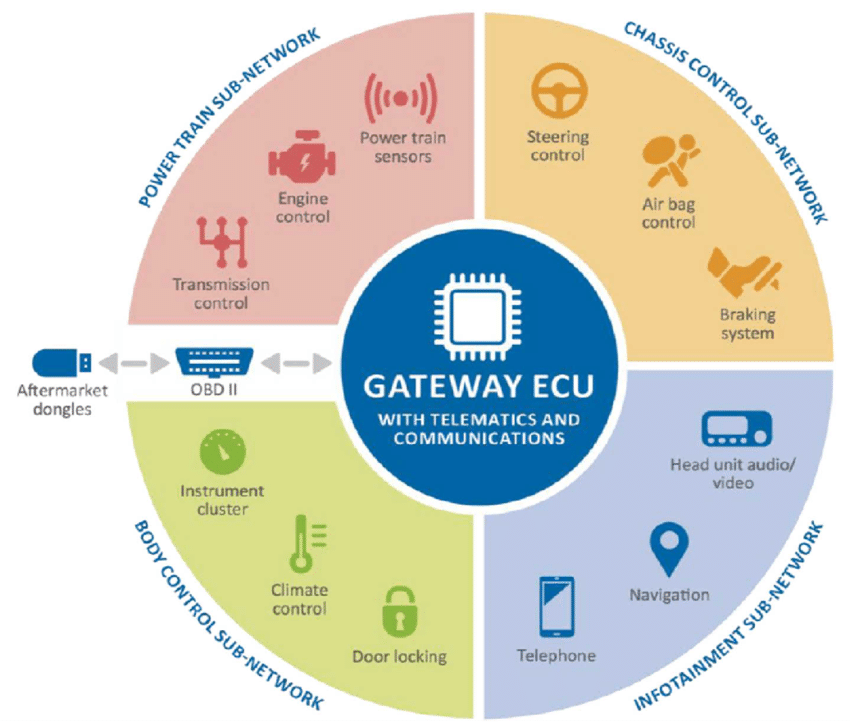
\includegraphics[width=\textwidth]{enisa.png}
	\caption{Typical intra vehicle network infrastructure \cite{Enisa}.}
    \label{fig:enisa}
\end{figure}
On top of their functional differences, these sub-networks often implement different network communications protocols. This means that there are multiple communication standards that are employed even within a single vehicle. The most common ones are: Controller Area Network (CAN), Local Interconnect Network (LIN), Media Oriented Systems Transport (MOST), FlexRay and LVDS \cite{Tuhoy}. Each of these protocols specifies how messages are exchanged within the appropriate sub-network. Their choice is based on the needs of a specific domain, as is illustrated in Table \ref{table:network_technologies} and \ref{table:network_technologies2}.
\begin{center}
\begin{table}[]
	\centering
	\begin{tabular}{|c|c|c|c|}
		\hline
		\rowcolor[HTML]{9B9B9B} 
		\textbf{Protocol} & \textbf{Bitrate} & \textbf{Medium} & \textbf{Protocol} \\ \hline
		LIN & 192 Kbps & Single Wire & Serial \\ \hline
		CAN & 1 Mbps & Twisted Pair & CSMA/CR \\ \hline
		FlexRay & 20 Mbps & Twister Pair/Optical Fibre & TDMA \\ \hline
		MOST &  150 Mbps & Optical Fibre & TDMA \\ \hline
		LVDS & 655 Mbps & Twisted Pair & Serial/parallel \\ \hline
	\end{tabular}
		\caption{An overview of different network technologies and their characteristics \cite{Tuhoy}.}
		\label{table:network_technologies}
\end{table}
\end{center}
\begin{table}[]
	\centering
	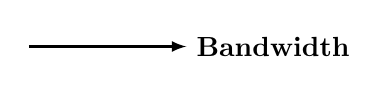
\begin{tikzpicture}[thick]
	\draw [black,  -latex] (0,6.5) -- (2,6.5) node [right] {\textbf{Bandwidth}} ;
	\end{tikzpicture}
	\begin{tabular}{cccccc}
		\cline{2-6}
		\multicolumn{1}{c|}{\textbf{LVDS}} & \multicolumn{1}{c|}{} & \multicolumn{1}{c|}{} & \multicolumn{1}{c|}{} & \multicolumn{1}{c|}{$\circ$} & \multicolumn{1}{c|}{$\circ$} \\ \cline{2-6} 
		\multicolumn{1}{c|}{\textbf{MOST}} & \multicolumn{1}{c|}{} & \multicolumn{1}{c|}{} & \multicolumn{1}{c|}{} & \multicolumn{1}{c|}{$\circ$} & \multicolumn{1}{c|}{} \\ \cline{2-6} 
		\multicolumn{1}{c|}{\textbf{FlexRay}} & \multicolumn{1}{c|}{} & \multicolumn{1}{c|}{$\circ$} & \multicolumn{1}{c|}{$\circ$} & \multicolumn{1}{c|}{} & \multicolumn{1}{c|}{} \\ \cline{2-6} 
		\multicolumn{1}{c|}{\textbf{CAN}} & \multicolumn{1}{c|}{$\circ$} & \multicolumn{1}{c|}{$\circ$} & \multicolumn{1}{c|}{$\circ$} & \multicolumn{1}{c|}{} & \multicolumn{1}{c|}{} \\ \cline{2-6} 
		\multicolumn{1}{c|}{\textbf{LIN}} & \multicolumn{1}{c|}{$\circ$} & \multicolumn{1}{c|}{} & \multicolumn{1}{c|}{} & \multicolumn{1}{c|}{} & \multicolumn{1}{c|}{} \\ \cline{2-6}
		& \textbf{Low} & \textbf{Real} &  &  & \textbf{Driver} \\
		& \textbf{Bandwith} & \textbf{Time} & \textbf{Safety} & \textbf{Infotainment} & \textbf{Assist} \\  
		& \textbf{Control} & \textbf{Control} & \textbf{Data} &  & \textbf{Cameras}         
	\end{tabular}
	\newline
	\caption{Mapping of traffic types to network technologies \cite{Tuhoy}.}
	\label{table:network_technologies2}
\end{table}
A critical component in vehicle networks is the gateway ECU. This component performs a frame or signal mapping function between two communication systems; allowing ECU's on different sub-networks, using distinct communication protocols, to exchange messages nonetheless. 
On top of acting as an intermediate between the different sub-networks of the vehicle, the gateway also acts as an entry point for OBD-II messages. Any message sent via the OBD-II port will be translated and forwarded by the gateway to the appropriate sub-network. It should come as no surprise that this component plays a crucial role when access control is introduced to the OBD-II interface.

\paragraph{Example: ABS}
Let's take a closer look at ABS to get a sense of how the intra vehicle network operates. ABS was designed to keep the wheels from locking up during braking. It consists of three main components: wheel speed sensors, a pump and a controller. Here's how it works \cite{wiki:ABS}:

\begin{itemize}
	\item The controller monitors the wheel speed sensors constantly (So each speed sensor periodically sends a message to the controller).
	
	\item The controller will recognize a wheel locking whenever it detects a rapid deceleration.
	
	\item Whenever the controller does detect a wheel locking up, it will use the pump (again by sending a message over the network) to regulate the pressure on the brake of that particular wheel, thereby keeping it from locking up.
\end{itemize}

\subsection{CAN}
\label{sec:can}

The CAN protocol has become a ubiquitous part of the automotive industry. In the context of internal vehicle networks, CAN messages have multiple purposes: First, there are informative messages, that are designed to transmit data from and to ECU's (e.g. the Anti-Lock System (ABS) broadcasting the speed of each wheel). Second, there are action messages that are designed to request another ECU to perform a specific action (e.g. the adaptive Cruise Control (ACC) module submitting a request for the brakes to be applied). Third, there are the diagnostic messages defined by the OBD-II protocol \cite{MillerB}. Naturally the last type of message is the focus of this paper. The following paragraphs are dedicated to the CAN protocol \cite{wiki:CAN,ISO11898-1}.

\subsubsection{Brief History} 
\label{subsec:can:briefhistory}

The history of CAN starts in 1983, when a couple of engineers at Bosch (soon aided by other engineers from Mercedes-Benz and Intel) start developing a new serial bus system for use in the automobile industry. It was not long before CAN was officially introduced at the SAE congress in Detroit as: 'Automotive Serial Controller Area Network'. The main characteristics of this new protocol were \cite{CANhistory}: 
\begin{itemize}
	\item An arbitration method that allows bus access to the message with the highest priority without delays.
	\item No need for a master node that is in charge of the bus.
	\item The identifier (ID) of these message identifies their content, not their destination or origin.
	\item This ID also determines the priority of the message within the network.
\end{itemize}
It didn't take long before the first CAN controller chips were developed in 1987 (by Intel and Philips respectively). The first official CAN specifications were standardised in the 90's, effectively paving the way for the CAN protocol to become an industry staple. To this day Bosh has been making sure that all CAN chips comply with their proposed standards, in an effort to avoid incompatible implementations. \footnote{For a comprehensive history of the CAN protocol see \cite{CANhistory}}

\subsubsection{Architecture}
\label{subsec:can:architecture}

A typical CAN network consists of a series of nodes connected by a two-wire bus. There are two physical CAN specifications: high speed CAN (see \cite{ISO11898-2}) and low speed (or fault tolerant) CAN (see \cite{ISO11898-3}). Every CAN node consists of:
\begin{itemize}
	\item CPU: This is effectively the 'brain' of the node, deciding what messages to send and taking the appropriate course of action whenever a message is received.
	\item Controller: in charge of reading and writing bits to and from the CAN bus.
	\item Transceiver: acts as in an intermediate between the bus and the controller, thereby translating between different signal levels.
\end{itemize}
This architecture specifies the minimum requirements of a CAN node. More often than not these nodes will also include a set of peripherals like sensors or actuators. It should be clear from this specification that this architecture applies to any common vehicle network (e.g. ECU's act as CAN nodes).

\subsubsection{CAN Frames}
\label{subsec:can:frames}
Since CAN is a message based protocol, it facilitates communication by transmitting short bursts of data called frames. There are four different types of CAN frames:
\begin{itemize}
	\item \textbf{Data frame:} used to transmit data with a specific identifier.
	\item \textbf{Remote frame:} used to request the transmission of data with a specific identifier.
	\item \textbf{Error frame:} transmitted whenever a node detects an error on the bus.
	\item \textbf{Overload frame:} transmitted by a node to include a delay between data or remote frame.
\end{itemize}
There are 2 frame formats: base frame format and the extended frame format. The only difference being that the extended frame format uses 29 identifier bits and the base frame format only uses 11. Table \ref{table:CANframeBase} and \ref{table:CANframeExtended} show the base and extended CAN frames respectively. The extended frame format is basically the same except for an additional identifier field (18 bits), immediately following the identifier extension bit (IDE) \cite{ISO11898-2,ISO11898-3}. 
\begin{table}[]
	\adjustbox{max width=\textwidth}{%
	\begin{tabular}{|c|c|c|c|c|c|c|c|c|}
		\hline
		\multirow{2}{*}{\textbf{SOF}} & \textbf{BASE} & \multirow{2}{*}{\textbf{RTR}} & \multirow{2}{*}{\textbf{IDE}} & \textbf{Control} & \multirow{2}{*}{\textbf{Data}} & \multirow{2}{*}{\textbf{CRC}} & \multirow{2}{*}{\textbf{ACK}} & \multirow{2}{*}{\textbf{EOF}} \\
		& \textbf{Identifier} & & & \textbf{Field} &  &  &  &  \\ \hline
		1 bit & 11 bits & 1 bit & 1 bit & 5 bits & 64 bits & 16 bits & 2 bits & 7 bits \\ \hline
	\end{tabular}
	}
	\caption{Base format CAN frame.}
	\label{table:CANframeBase}
\end{table}
\begin{table}
	\adjustbox{max width=\textwidth}{%
	\begin{tabular}{|c|c|c|c|c|c|c|c|c|c|c|}
		\hline
		\multirow{2}{*}{\textbf{SOF}} & \textbf{BASE} & \multirow{2}{*}{\textbf{SRR}} & \multirow{2}{*}{\textbf{IDE}} & \textbf{Ext.} & \multirow{2}{*}{\textbf{RTR}} & \textbf{Control} & \multirow{2}{*}{\textbf{Data}} & \multirow{2}{*}{\textbf{CRC}} & \multirow{2}{*}{\textbf{ACK}} & \multirow{2}{*}{\textbf{EOF}} \\
		& \textbf{ID} & & & \textbf{ID} & & \textbf{Field} &  &  & & \\ \hline
		1 bit & 11 bits & 1 bit & 1 bit & 18 bits & 1 bit & 6 bits & 64 bits & 16 bits & 2 bits & 7 bits \\ \hline
	\end{tabular}
	}
	\caption{Extended format CAN frame.}
	\label{table:CANframeExtended}	
\end{table}
\subsubsection{Data Transmission}
\label{subsec:can:data_transmission}

The operation of the CAN protocol is pretty straightforward: a node transmits a message with a specific ID on the bus. Any node connected to the same bus is able to receive the message, but only the nodes that are listening for this specific ID will take action. It is worth stressing again that the ID is used to identify the content, not the sender or receiver. As a matter of fact CAN does not provide any way of authenticating the sender or receiver, which results in various security related difficulties (see Section \ref{subsec:can:security_issues}). Aside from identifying the content, this ID is also used to solve the issue of message arbitration. CAN is a carrier sense multiple access protocol; each nodes observes the bus before transmitting data on it. If a node detects that the bus is in use, it waits for some time before trying again. However, this does not prevent multiple nodes from starting a data transfer at the same time. These situations were avoided with the introduction of bit wise message arbitration, which is discussed in the next section \cite{CANarbitration}.

\subsubsection{Message Arbitration}
\label{subsec:can:message_arbitration}

Whenever two or more nodes initiate a transmission on the bus at the same time, a bit wise message arbitration is performed. Every bit of the message ID can be either 1 or 0. The CAN specifications use the term dominant (logical 0) and recessive (logical 1). These terms originate from the fact that whenever more than one bit is simultaneously written to the bus, and one of these is dominant; the dominant bit 'wins', meaning a logical 0 will be seen on the bus. Whenever a node transmits a logical 1 but sees a logical 0; it realizes that there is a contention and re-queues its message for later transmission. Since the identifier is transmitted at the start of the CAN frame, the node with the numerically lowest identifier transmits more zeros at the start of the frame, and that is the node that wins the arbitration. Thus, messages with lower ID's have priority over messages with higher ID's. The decision to identify messages by their content (instead of their sender or receiver) is motivated by the fact that more important messages (e.g. errors) can be given a very low id, thereby ensuring they are prioritised \cite{ISO11898-2,ISO11898-3}. 

\subsubsection{Layering}
\label{subsec:can:layering}

It is common practice to decompose networking protocols into different abstract layers. This is done to simplify their design and make modularisation easier \cite{wiki:ProtocolStack}. In the case of the CAN protocol the layers are \cite{ISO11898-2,ISO11898-3}:

\begin{itemize}
	\item \textbf{Application layer:} OBD-II, CANOpen, etc.
	\item \textbf{Object layer:} message filtering and status handling.
	\item \textbf{Transfer layer:} error detection, message arbitration, bit timing, etc.
	\item \textbf{Physical layer:} signal voltages, pin-out configuration, etc.
\end{itemize}

\subsubsection{Security Issues}
\label{subsec:can:security_issues}

The CAN protocol has a number of inherent vulnerabilities that are common to any implementation. The most obvious and important ones are:

\begin{itemize}
	\item \textbf{Eavesdropping:} CAN frames are both physically and logically (no destination address) broadcasted on the network. This means that a malicious node on the bus can snoop on all communications; or even worse, send packets to any other node on the network \cite{Kosher}. 
	
	\item \textbf{No authentication:} CAN frames do not have source identifier fields, so there is no way for any node to be aware of the source of any messages it receives. This means that any compromised component (or any other form of unsanctioned access to the CAN bus for that matter) can inject arbitrary messages. The system has no way of knowing these messages were not sent by the appropriate component \cite{Kosher,CANissues}.
	
	\item \textbf{No encryption:} Speed and timing are deemed more important to the safety and performance of the vehicle than data security \cite{Klinedinst05}. A clear result of this is the decision to omit any encryption capabilities. This is because of the limited  computational power of ECU's, that makes it difficult to implement robust cryptographic algorithms \cite{CANissues}.  
	
	\item \textbf{Susceptibility to Denial of Service (DoS):} This problem arises mainly from the protocol's message arbitration method. Any malicious node can effectively spam the bus with high priority messages (only zeroes as ID), causing all other nodes to back off (no protection against "babbling idiots") \cite{Kosher,Pike15}.
	
	\item \textbf{Not Byzantine fault tolerant:} In most distributed systems, malicious attacks and software errors can cause a node to exhibit Byzantine (i.e. arbitrary) behaviour \cite{Byzantine}. Because of the distributed nature of any CAN system, there is imperfect information on whether a component has failed (or has been compromised by attack) or not. This could result in situations where the entire system fails, since a common consensus cannot be reached \cite{wiki:ByzantineFault}.\footnote{For more information on Byzantine faults, and how it is tolerated in a system see \cite{Byzantine} and \cite{wiki:ByzantineFault}.}
	
\end{itemize}
We refer te reader to \cite{ISO11898-2} and \cite{ISO11898-3} for more information on the CAN protocol.

\subsection{OBD-II}
\label{sec:obd}

\subsubsection{Brief History}
\label{subsec:obd:brief_history} 

\cite{ISO15031-1,ISO15031-2,ISO15031-3,ISO15031-4,ISO15031-5,ISO15031-6,ISO15031-7}

There have been a lot of different proprietary automotive diagnostics systems introduced over the years, before a standard arrived with the introduction of OBD-II. This brief history, cited from \cite{OBDhistory}, does an excellent job of concisely explaining how OBD-II came to be:

\begin{displayquote}
	The origins of OBD-II actually date back to 1982 in California, when the California Air Resources Board (ARB) began developing regulations that would require all vehicles sold in that state starting in 1988 to have an onboard diagnostic system to detect emission failures. The original onboard diagnostic system (which has since become known as OBD-I) was relatively simple and only monitored the oxygen sensor, exhaust gas circulation system, fuel delivery system and engine control module.
	
	OBD-I was a step in the right direction, but lacked any requirement for standardization between different makes and models of vehicles. You still had to have different adapters to work on different vehicles, and some systems could only be accessed with costly "dealer" scan tools. So when ARB set about to develop standards for the current OBDII system, standardization was a priority: a standardized 16-pin data link connector (DLC) with specific pins assigned specific functions, standardized electronic protocols, standardized diagnostic trouble codes (DTCs), and standardized terminology.
	
	Another limitation of OBD-I was that it couldn't detect certain kinds of problems such as a dead catalytic converter or one that had been removed. Nor could it detect ignition misfires or evaporative emission problems. Furthermore, OBD-I systems would only illuminate the MIL light after a failure had occurred. It had no way of monitoring progressive deterioration of emissions-related components. So it became apparent that a more sophisticated system would be required. The California Air Resources Board eventually developed standards for the next generation OBD system, which were proposed in 1989 and became known as OBD-II. The new standards required a phase-in starting in 1994. The auto makers were given until the 1996 model year to complete the phase-in for their California vehicles.
	
	Similar standards were incorporated into the federal Clean Air Act in 1990 which also required all 49-state vehicles to be OBD-II equipped by 1996 -- with one loophole. The OBD-II systems would not have to be fully compliant until 1999. So some 1996 OBD-II systems may lack one of the features normally required to meet the OBD-II specs, such as the evaporative emissions purge test.
\end{displayquote}

\subsubsection{Design Goals} 
\label{subsec:obd:design_goal}

OBD-II is a specification that has been introduced to allow for self diagnostic and reporting functionality for ECU's inside a vehicle, and has been mandatory in every car produced in the united states since 1996 \cite{wiki:OBD}. It allows users (testers, developers, repairmen, etc.) to query ECU's about diagnostics information, in order to perform a detailed analysis of the vehicles internal systems. Specifically, the goals of OBD-II upon introduction were: 
\begin{itemize}
	\item Standardisation: information is communicated in a standardized format to allow for 1 tool to be used on many vehicles.
	\item Certification: Every vehicle manufacturer is required to apply for certification, which includes submitting a detailed description of how the OBD-II protocol was implemented.
	\item Help lowering emissions by identifying emission controls in need of repair.
\end{itemize} 
The system can also be very useful in a number of other situations: a repairman looking for a specific component that is to be repaired, an employee at the factory testing all components before the vehicle is ready to be sold, a policeman analysing a vehicle after a crash to determine what caused the accident, a software developer testing the operation of a newly developed ECU, etc. 

\subsubsection{DLC}
\label{subsec:obd:dlc}

To allow a user to communicate with the vehicle's internal network, OBD-II introduces the data link connector (DLC). The DLC is a 16-pin hardware interface (although only 9 pins are specified by the standard) that is generally found close to the steering wheel (by law it is required to be installed within 0.61 m of the steering wheel) \cite{wiki:OBD}. There are 2 basic types of connectors: Type A as seen in Figure \ref{fig:typeA} (using a 12V power supply) and Type B as seen in Figure \ref{fig:typeB} (using a 24V power supply). The design of the two connector types prevents the insertion of a type A male plug into a type B female socket. There are multiple ways for a user to connect to the the OBD-II DLC:
\begin{itemize}
	\item A standard diagnostic scanning tool, which is a dedicated device that consists of a small hand-held module (equipped with a small screen and some buttons), connected to a male DLC (The DLC inside the vehicle is always female).
	
	\item An advanced Diagnostic scanning tool that includes a DLC-connector with wifi/Bluetooth compatibility, allowing for remote diagnostics via smartphone or PC.
	
	\item A DLC-connector with a USB adapter, allowing access via dedicated software on a PC. Since 2014, all new cars in the US support the SAE J2534 "PassThru" standard, which is a Windows application programming interface (API) that provides a standard way to communicate with a car's internal buses \cite{Kosher}.\footnote{For more information on SAE J2534, see the full API reference at: \url{https://tunertools.com/prodimages/DrewTech/Manuals/PassThru\textunderscore API-1.pdf}}
	
	\item A data logger, which is designed to capture real-time data while the vehicle is in operation.
\end{itemize}

\begin{figure}[h]
	\centering
	
\includegraphics{typeA.png}
	\caption{Type A female connector \cite{wiki:OBD}.}
	\label{fig:typeA}
\end{figure}

\begin{figure}[h]
	\centering
	
\includegraphics{typeB.png}
	\caption{Type B female connector \cite{wiki:OBD}.}
	\label{fig:typeB}
\end{figure}

\subsubsection{PID and DTC}
\label{subsec:obd:pid}

OBD-II introduces parameter identification numbers (PID) in ISO15031-5 \cite{ISO15031-5}, which are codes used to identify and query data. Besides the PID's offered by this standard (suitably called the standard PID's), a lot of manufacturers will implement their own model-specific PID's. Two types of data that can be queried. First, there is raw engine data like fuel pressure, air intake temperature, engine rounds per minute, etc. Second, there are diagnostic trouble codes (DTC). These codes consist of five characters, encoded in two bytes of data. With the help of the appropriate OBD-II DTC table, these codes can be interpreted to identify and locate specific problems \cite{wiki:PID}.

\subsubsection{ISO-TP}

The PID's introduced in the previous paragraph need to transmitted to the appropriate ECU. This is where the signalling protocol comes in. Five different signalling protocols are permitted for transmitting OBD-II messages. However, ISO-TP, which is introduced in ISO15765 \cite{ISO15765-2:2016}, is the most widely implemented. This is because since 2008, all new vehicles sold in the US are required by law to implement this protocol. ISO-TP was designed in accordance with the Unified Diagnostic Services (UDS) specified in ISO14229 \cite{ISO14229}. It allows a message size of up to 4095 bytes, and facilitates this by spreading out the message over multiple CAN frames. The format of these messages is left unchanged, thus allowing 8 bytes of data per frame. However, the first data byte is used for Protocol Control Information (PCI), resulting in only 7 bytes of actual data being transmitted with each frame. The four most significant bits of the PCI indicate the PCI type. There are four types of ISO-TP frames:
\begin{itemize}
	\item \textbf{Single Frame (SF):} Whenever the message is no more than 7 bytes long, it will fit into a single ISO-TP frame. Upon reception of a SF, the receiving party knows the entire message was transmitted.
	
	\item \textbf{First Frame (FF):} This frame is used to let the receiver know that the message is longer than 7 bytes, thereby requiring multiple frames (Multi-Frame format). The FF uses two bytes of data for PCI: the four most significant bits are used to indicate the PCI type, and the 12 least significant bits are used to indicate the size of the complete message, allowing the receiver to know how many more frames to expect.
	
	\item \textbf{Flow Control Frame (FC)}: Upon reception of a FF, the receiver will respond by transmitting a FC. This frame contains synchronisation and buffering information, allowing the sender to transmit frames at the appropriate frequency, as well as when to expect (i.e. after how many successful transmissions) another FC frame update.
	
	\item \textbf{Consecutive Frame (CF)}: When transmitting a message in multi-Frame Format, consecutive messages will be sent until the entire message was transmitted. The four least significant bits of a CF implement a counter to allow the receiver to correctly assemble the original message.
\end{itemize}
Figure \ref{fig:ISO-TP} shows the operation of ISO-TP when transmitting a message in Multi-Frame format. Notice the fact that this sequence can include the transmission of multiple FC's. This is because the receiver might be limited in the amount of CAN buffers available. Every FC will contain information on how many messages to send before these buffers are full.

\begin{figure}[h]
	\centering
	\fbox{
		\procedure{ISO-TP Multi Frame Format}{%
			\textbf{Sender}  \<\< \textbf{Receiver} \\
			\< \sendmessageright{top=First Frame} \<\\
			\< \sendmessageleft{top=Flow Control Frame} \<\\
			\< \sendmessageright{top=Consecutive Frame} \<\\
			\< \sendmessageright{top=Consecutive Frame} \<\\
			\vdots \< \< \vdots \\
			\< \sendmessageleft{top=Flow Control Frame} \<\\
			\< \sendmessageright{top=Consecutive Frame} \<\\
			\< \sendmessageright{top=Consecutive Frame} \<\\
			\vdots \< \< \vdots \\
		}
	}
	\caption{ISO-TP}
	\label{fig:ISO-TP}
\end{figure} 

\subsubsection{Use Case}
Typically, ODB-II is used like this (CAN as signalling protocol): First, the user enters the PID of the data (s)he wants to query into a diagnostic tool. Second, this data is packaged in a CAN frame and sent over the CAN-bus. Third, the ECU that is responsible for the data identified by the PID in the message recognizes it as it's own, and transmits a CAN frame containing the requested data. Fourth, the diagnostic tool recognizes the response and displays the data to the user \cite{wiki:PID}. The OBD-II port can also be used to upgrade the ECU's firmware or to perform a myriad of other diagnostic tasks.





\subsubsection{Security Issues}
\label{subsec:obd:security_issues}

It is a well-known fact that the automotive industry has always considered safety a critical engineering concern \cite{Dyer}. Unfortunately, it is unclear whether developers (especially concerning the internal network) have considered the security in their design. It seems this is not the case because of three reasons. First, as is asserted in \cite{MillerB}, 'there is no inherent support for addressing, encryption or authentication'. Second, most of the networks and ECU's were designed when access to the bus required physical access to the vehicle, therefore security was not a primary concern. Third, speed and timing are considered more important to the safety of the vehicle than the security of transmitted data \cite{Klinedinst05}. This vulnerability is worsened by the fact that the attack surface of modern automobiles is growing swiftly, as more sophisticated services and communications features are incorporated into vehicles \cite{Kosher}. The OBD-II specification is one of these, since its interface provides direct access to the internal vehicle network. This allows malicious agents to easily construct and insert CAN messages to alter the vehicle's behaviour, as has been frequently demonstrated by Charlie Miller and Chris Valasek's exploits \cite{MillerA, MillerB, MillerC}. The goal of this research paper is to design a solution that prevents malicious agents from mounting attacks via the OBD-II interface, while still allowing for the system to function properly (i.e. performing diagnostics and maintenance). 

\section{Preliminaries}
\label{chap:preliminaries}

This section serves as a technical primer to all the security related software solutions that are employed in this paper. The reader should keep in mind that the selection of algorithms and systems presented here is far from comprehensive; only those that are relevant to the solution presented in this paper are discussed.

\subsection{ECU Microcontrollers}
\label{sec:microcontrollers}

An ECU is an embedded computer that is designed to perform a specific function. The core of any ECU is a small computer on an integrated circuit called a microcontroller. A microcontroller consists of one or more central processing units (CPU) along with memory and programmable input/output peripherals. There a couple of characteristics of microcontrollers that are touched upon in the course of this paper, so a description of these is given next:

\begin{itemize}
	\item \textbf{Word size:} The word size of a microcontroller (or any computer for that matter) is the natural unit of data used by a particular processor. A word is a fixed-sized piece of data handled as a single unit by the instruction set or the hardware of the processor. The number of bits in a word is an important characteristic of any microcontroller. Within the context of ECU's, word sizes of 8 bits (e.g. driver information), 16 bits (e.g. vehicle control) and 32 bits (e.g. power train) are most common \cite{ECU}.
	
	\item \textbf{Clock rate:} The clock rate of a CPU refers to the rate at which it processes words of data. it is used as an indicator of the processor's speed. It is measured in clock cycles per second or hertz (Hz). 
	
	\item \textbf{Memory:} There are two basic types of memory: 
	\begin{itemize}
		\item \textbf{Data Memory}: Data memory is where variables and all intermediate calculations are stored by the CPU. It is generally implemented by RAM\footnote{random access memory (RAM) is a type of memory where individual data can be read or written in almost the same amount of time irrespective of the physical location of data inside the memory.}. This data is often volatile, meaning the data is lost when power is removed.
		
		\item \textbf{Program memory}: Program memory is where the application is stored, i.e. the code itself. This type of memory is implemented using non-volatile storage technologies like ROM \footnote{Read-only memory (ROM) is a type of non-volatile memory where the data stored can not be modified (or where it is considered very difficult to do so).}, EPROM\footnote{erasable programmable read-only memory (EPROM) is a non-volatile type of memory that can be erased (by exposing the chip the ultraviolet light) and reprogrammed.}, EEPROM\footnote{Electrically erasable programmable read-only Memory (EEPROM) is a type of non-volatile memory that can be erased and reprogrammed electronically.} or Flash Memory\footnote{Flash memory is type of EEPROM  that can be electrically erased and reprogrammed much faster than regular EEPROM chips by using large erase blocks.}.
	\end{itemize}
	
	\item \textbf{Serial Communications Interfaces:} Serial communications is a way of communication in computer networks where bits are transmitted one bit at a time (e.g. CAN). This is in contrast to parallel communications where a link is used with several parallel channels, allowing multiple bits to be sent at the same time (e.g. USB). Most microcontrollers offer dedicated hardware allowing for easy communication with other devices (e.g. CAN controller).
	
	\item \textbf{Others:} Most microcontrollers offer various other hardware like: a timer, an analog-to-digital convertor (ADC) that allows for an analog signal (like the output of a sensor) to be transformed into a digital signal, a clock generator, etc.
\end{itemize}

\subsection{Role-Base Access Control}
\label{sec:RBAC}

Role-based access control (RBAC) is a well-defined way of restricting system access to authorized users. It especially useful in large enterprises where roles are created for various job functions. Each role is assigned the necessary permissions to interact with a secured system (e.g. the company database, the local private network, development software, etc). The idea is that a worker is assigned a role based on what (s)he requires to do their job, and nothing more. To avoid that workers are granted permissions they do not need. There are two basic types of RBAC \cite{wiki:RBAC}.

\begin{itemize}
	\item \textbf{Mandatory Access Control:} In a system where mandatory access control (MAC) is a enforced, only the administrator of the system is able to create and assign roles. This is done by defining a security policy that users are unable to override or alter. The administrator of the system is called the security policy administrator.
	
	\item \textbf{Discretionary Access Control:} When discretionary access control (DAC) is enforced, it is up to the users themselves to make policy decisions and/or assign security attributes.
\end{itemize}

\subsubsection{Permission Table}
\label{subsec:permissions_table}

RBAC systems are generally implemented by introducing a permission table. This table is a software representation of the agreed-upon security policy. There is an entry in this table for each permission that can be assigned (e.g. access to files, permission to create/delete folders, etc). Every field of each entry corresponds with a role, and whether this role is granted the corresponding permission. 

\subsection{Public Key Cryptography}
\label{sec:PKC}

\subsubsection{Cryptography} 
\label{subsec:cryptography}

The primary goal of cryptography in general is to allow for secure communication between two parties. This means that protocols are designed that prevent third parties or the public in general from reading private messages. This is done by encrypting the message, which consists of converting the information from a readable state to apparent nonsense. Only the intended recipient should be able to restore the information to it's original form, which is called decryption. To allow for this to work, the procedure of encryption and decryption should only be possible by the sender and the receiver respectively. Generally this procedure consists of two parts. First, there is the cypher, which is the algorithm that does the actual conversion. Second, there's the secret key, which is used by the cipher together with the input (plaintext) to create the encrypted output (ciphertext). The main advantage of this architecture is that the chosen cipher can be made public, as long as the key is kept secret. The receiver of the secret message, who is in possession of the same secret key, runs the same cipher in reverse with the secret key and the ciphertext as inputs, yielding the original plaintext \cite{wiki:Cryptography}.

\subsubsection{Symmetric vs Asymmetric}
\label{subsec:symmetric_vs_assymetric}

The procedure outlined above is called symmetric key cryptography, since both parties are in possession of the same secret key. The disadvantage here is that these keys need to be securely exchanged beforehand (e.g. via a secure channel) to allow for secure communications. Asymmetric (or public key) cryptography offers a solution to this problem. In this case, a key pair is created where each one serves a specific function. The first one is called the private key, which is meant to be kept secret at all times by the owner. The second one is called the public key, which is disseminated widely to the public. The idea is that if someone wants to send an encrypted message to the owner of the private key, (s)he looks up the corresponding public key (generally found online); uses the public key to encrypt a message, and sends this message to the owner. Since only the owner is in possession of the corresponding private key, only (s)he is able to decrypt the message.

\subsection{Key Exchange} 
\label{sec:key_exchange}

The specifications of symmetric and asymmetric encryption are sound. However they both rely on both parties being in possession of the right key. In the case of asymmetric encryption this is easy: The owner generates a new public/private key pair, stores the private key in a safe location, and distributes the corresponding public key on the Internet. Anyone who wants to securely communicate with the owner only has to look up the corresponding public key. This procedure does not apply to symmetric encryption however, since only the sender and receiver should be in possession of the secret key. One way of safely distributing the key is to use a secure communications channel. Examples of this are: a text message, a phone call, physically handing over the key, sending a letter, etc. However, it is clear that in most situations this method simply will not do, since it requires significant effort before a secure communication session can be established. Two more realistic alternatives exist: using asymmetric keys to establish a session key and key exchange algorithms. Both will be discussed in turn next.

\subsubsection{Session Keys} 
\label{subsec:session_keys}

The free distribution of public keys can be leveraged to establish a new temporary shared key, also called a session key. If Alice has an asymmetric key pair already established, and Bob wishes to establish a shared secret key with Alice; bob only has to look up Alice's public key, generate a new session key, encrypt the new session key using Bob's public key, and send it to Alice. Alice can then decrypt the session key using her private key. In the end both parties are in possession of the new session key, and a secure communication can be established. Now, the reader might wonder why it is necessary to establish a session key, since secure communications could also be performed using asymmetric keys (granted they both have an asymmetric key pair). This is mainly due to performance. Asymmetric encryption requires significantly longer keys to guarantee the same level of security, and the corresponding procedures (e.g. encryption, decryption, signing, etc.) take significantly longer to perform. Therefore, it is often beneficial to establish a session key, instead of repeatedly using asymmetric keys.

\subsubsection{Key Exchange Algorithms} 
\label{subsec:key_exhange_algorithms}

Key exchange algorithms allow two parties that have no prior knowledge of each other to establish a shared secret key over an insecure channel. The most famous example of such an algorithm is the Diffie-Hellman key exchange method \footnote{for more information on Diffie-Hellman see \cite{wiki:DH}}. These algorithms typically rely on computationally hard to solve mathematical problems such as the discrete logarithm.

\subsection{Authentication} 
\label{sec:authentication}

Besides protecting messages from being read by a third party, the recipient of the message might also want certainty on who sent it in the first place, as well as knowing that the message has not been tampered with. In other words the recipient wants to guarantee the integrity of the message, on top of authenticating the sender. Fortunately asymmetric and symmetric cryptography offer solutions in the form of digital signatures and message authentication codes respectively. Before going into this however, it is necessary to first take a look at hash functions.

\subsubsection{Hash functions} 
\label{subsec:hash_functions}

A hash function is used to map data of arbitrary size to data of a fixed size. The values returned by a hash function are called hash values, hash codes, digests, or simply hashes. For a hash function to be useful in cryptography (also called a cryptographic hash function) it has to possess the following properties \cite{wiki:Hash}:

\begin{itemize}
	\item The same message always results in the same hash value.
	\item The hash function does not take long to perform.
	\item It is infeasible to reconstruct the original message from the hash value.
	\item Two similar messages have widely varying hash values.
	\item it is infeasible to find two different messages with the same hash value.
\end{itemize}

\subsubsection{Digital Signatures} 
\label{subsec:digital_signature}

A digital signature is used to verify the authenticity of digital messages. The principle is simple: If Alice wants to send an authenticated message to Bob, she will first sign the message using her private key. She then sends the message together with the generated signature to Bob. Bob can then check the authenticity of the message by verifying the signature using Alice's public key. If the verification was successful, Bob can safely assume 2 things: the message was sent by Alice (since she is in possession of the corresponding private key) and the message was not tampered with in transit (since in that case the signature would no longer match the message, resulting in a failed verification). Two additional algorithms are required: a signing algorithm and a signature verification algorithm. Ideally the signing algorithm would produce a signature of the same size, regardless of the size of the original message. This is where cryptographic hash functions come in, since they possess this property. Generally the message will first be hashed to a fixed size, before being processed by the signing algorithm. Besides guaranteeing a fixed sized output, this also improves the overall efficiency \cite{wiki:DigitalSignature}.

\subsubsection{MAC's} 
\label{subsec:MAC}
a message authentication code (MAC) serves the same function as a digital signature algorithm. Namely, guaranteeing the authenticity and integrity of a transmitted message. The main difference is that MAC's are based on symmetric keys rather than asymmetric keys. 

\subsection{Authenticated Key Agreement}
\label{sec:AK}

As will become apparent in Section \ref{subsec:authenticated_key_agreement_procedure}, it is generally advised to combine authentication and shared secret establishment into a single procedure. This is called authenticated key agreement (AK). In AK systems both parties are mutually authenticated while a shared secret is established. It is only assured that both parties are able to generate the shared secret, not that this secret was actually computed. A protocol that also guarantee to both parties that the other party actually computed the secret is called authenticated key agreement with key confirmation (AKC) \cite{Blake-Wilson}.

\subsection{Security Level}
\label{sec:security_level}

The security level of a cryptographic primitive (e.g. a hash function, a key, a cipher) refers to the difficulty for any attacker to break it. The security level is usually expressed in bits, where  an $n$-bit security level indicates that an attacker would have to perform (at least) $2^n$ operations to effectively crack the cryptographic primitive. It is very useful when comparing between different cryptographic algorithms, which will be done frequently during the course of this paper.

\section{Chosen Security Systems}
Previously an attempt was made to explain the basic principles behind the security systems that will be implemented in this paper. A multitude of various approaches to these systems exist however. The difference between them is mostly down to the mathematical structure of the approach, as well as the effect this has on efficiency and performance when they are implemented. This section will give an overview of the different implementations that were chosen for this paper, as well as motivating why these decisions were made.

\subsection{Elliptic Curve Cryptography}
\label{subsec:ECC}

There exist a couple of well-known public key cryptography technologies. The basic principle behind all of them is the use of functions that are easy to perform in one direction, but where the inverse is far more difficult (these are called trapdoor functions). Take prime multiplication for example: if we take two prime numbers $p$ and $q$, it is quite easy to calculate the product $n=pq$. However the factorisation of $n$ into $p$ and $q$ is way more difficult, especially when these numbers are significantly large. This is called the factoring problem and is the backbone of the Rivest Shamir Adleman (RSA) cryptosystem. This property is then leveraged to make it difficult to calculate the private key from the public key, while calculating the public key from a random private key is rendered trivial. The problem with RSA however is that it requires very long key sizes (currently the minimal recommended key size is 2048 bits \cite{RSAlength}), and the corresponding procedures are very slow \cite{wiki:RSA}. This wouldn't be a problem if the enough processing capacity were available. However, for the typical microcontroller found in ECU's this is not the case. It was shown in \cite{Sethi} that using the RSA digital signature operation (with a key size of 2048 bit) in a typical 8-bit microcontroller (the ATmega328, which has a clock speed of 16 MHz, 2 kB of RAM, and 32 kB of flash memory), takes roughly 26 minutes to complete. Luckily elliptic curve cryptography offers a solution to this.

\paragraph{ECC} Elliptic curve cryptography (ECC) is an approach to public-key cryptography based on the algebraic structure of elliptic curves over finite fields instead of plain Galois fields, like most other non-EC based algorithms. Where RSA was based on the difficulty of the factorisation problem, ECC is based on the discrete logarithm of a random elliptic curve element with respect to a publicly known base point, which is called the elliptic curve discrete logarithm problem (ECDLP) \cite{Siddiqui}. The advantage of ECDLP is that it is way more difficult to solve than the factorisation problem of RSA. This means that for the same key size, ECC is more secure than RSA (i.e. assures a greater security level). In other words, when using ECC we can use smaller key sizes, while still guaranteeing the same level of security. Running the elliptic curve digital signature algorithm (ECDSA) on the same microcontroller as before, with a curve that guarantees the same level of safety as an RSA 2048 bit key, takes roughly 6 seconds to complete. This is a significant improvement over the 26 minutes it took RSA \cite{Sethi}.

\subsubsection{ECDSA} 
\label{subsubsec:ecdsa}

The elliptic curve digital signature algorithm (ECDSA) is the default elliptic curve variant of digital signatures. 

\subsubsection{ECDH} 
\label{subsubsec:ecdh}

Besides using ECC for digital signatures with ECDSA, another ECC based protocol that is chosen in this paper is elliptic curve Diffie-Hellman (ECDH). Like normal Diffie-Hellman it is used when two communicating parties wish to establish a shared secret (or session key) over an insecure channel. First, the two communication parties agree on the elliptic curve they will use. Second, they both generate an ECC key pair. Third, they exchange their public keys. In the last step they both use their own private key, together with the public key they received to generate the same secret value. Any third party listening on the channel only knows both public keys, which is not enough to easily calculate the shared secret since they would have to solve the ECDLP.

\subsubsection{ECDHE\_ECDSA} 
\label{subsubsec:ecdh_ecdsa}

As mentioned in Section \ref{sec:AK} and illustrated in Section \ref{subsec:authenticated_key_agreement_procedure}, it is a common practice to combine authentication and shared secret establishment into a single procedure. In \cite{RFC4492} multiple methods are proposed that perform ECDH, while also providing authentication using elliptic curve digital signatures. One of these methods is called ECDHE\_ECDSA and is illustrated in Figure \ref{fig:ECDH2}. The extra E in ECDHE comes from th fact that this procedure uses "ephemeral" (i.e temporary) keys. Two communicating parties (Alice and Bob) are both in possession of an elliptic curve private/public key pair: $Pb_a$,$Pr_a$ (Alice) and $Pb_b$,$Pr_b$ (Bob). Alice signals to Bob that she wishes to initiate a ECDHE\_ECDSA sequence by sending a 'hello' message to Bob. Bob then creates a new ephemeral elliptic curve key pair: $Pb_{bE}$,$Pr_{bE}$, signs the new ephemeral public key using his own private key: Sig($Pb_{bE}$,$Pr_b$), and sends this to Alice. She will first verify the signature: Ver(Sig,$Pb_{b}$), thus authenticating Bob to Alice. After which she will also generate her own ephemeral key pair using the same curve as Bob: KGen($Pb_{aE}$,$Pr_{aE}$), before signing the new public key and sending it to Bob: Sig($Pb_{aE}$,$Pr_a$). Bob will then in turn verify the signature using Alice's public key: Ver(Sig,$Pb_{a}$). Alice and Bob are now both in possession of each other's ephemeral public keys, to use ECDH to generate a shared secret: $K$=ECDH($Pr_{aE}$,$Pb_{bE}$) for Alice and $K$=ECDH($Pr_{bE}$,$Pb_{aE}$) for Bob. The attentive reader might wonder why these ephemeral key pairs are generated at all. why not use the pre-existing key pairs $Pb_a$,$Pr_a$ and $Pb_b$,$Pr_b$ to generate the shared secret. This is because introducing these ephemeral keys guarantees perfect forward secrecy (PFS)\footnote{Perfect forward secrecy is guaranteed when a posteriori leak of one of the used private keys (e.g. $Pr_a$ and $Pr_b$ in figure \ref{fig:ECDH2}) does not result in the communication session (i.e. the session key) being compromised.}.


\begin{figure}[h]
	\centering
	\fbox{
		\procedure{ECDHE\_ECDSA}{%
			\textbf{Alice}  \<\< \textbf{Bob} \\
			\text{$Pb_a$,$Pr_a$} \<\< \text{$Pb_b$,$Pr_b$} \\
			\< \sendmessageright{top=\text{hello}} \<\\
			\<\< \text{KGen($Pb_{bE}$,$Pr_{bE}$)} \\
			\< \sendmessageleft{top=\text{Sig($Pb_{bE}$,$Pr_b$)}} \<\\
			\text{Ver(Sig,$Pb_{b}$)} \<\< \\
			\text{KGen($Pb_{aE}$,$Pr_{aE}$)} \<\< \\
			\< \sendmessageright{top=\text{Sig($Pb_{aE}$,$Pr_a$)}} \<\\
			\<\< \text{Ver(Sig,$Pb_{a}$)} \\
			\text{$K$=ECDH($Pr_{aE}$,$Pb_{bE}$)} \<\< \text{$K$=ECDH($Pr_{bE}$,$Pb_{aE}$)} \\
		}
	}
	\caption{ECDHE\_ECDSA}
	\label{fig:ECDH2}
\end{figure} 

\subsection{SHA-256 and SHA-512} 
\label{subsec:sha}

A lot of cryptographic procedures require the data to be hashed first; the implementation of this research paper is certainly no exception. The choice was made to use the secure hash algorithm (SHA) family of hash functions. SHA constitutes a large set of cryptographic hash functions that were designed by the United States National Security Institute (NSA). There exist four distinct sets of SHA \cite{wiki:SHA}:

\begin{itemize}
	\item \textbf{SHA-0}: Published in 1993, was withdrawn shortly after publication because of a significant flaw.
	
	\item \textbf{SHA-1}: Published in 1995 as a replacement to SHA-0. It has been considered insufficiently secure since 2011 \cite{Stevens}.
	
	\item \textbf{SHA-2}: Published in 2001, consists of six hash functions with hash values that are 224, 256, 384 or 512 bits in size: SHA-224, SHA-256, SHA-384, SHA-512, SHA-512/224 and SHA-512/256 \cite{RFC6234}.
	
	\item \textbf{SHA-3}: Pubished in 2015, subset of the broader cryptographic primitive family Keccak, conists of the following hash functions: SHA3-224, SHA3-256, SHA3-384 and SHA3-512 \cite{SHA3}.
\end{itemize} 
While the SHA-3 hash functions were an obvious candidate, simply because they are newer and deemed more secure, the choice was made to work with the SHA-2 hash functions instead. This is because SHA-2 libraries are better when it comes to performance \cite{Murvay}.

\subsection{HMAC} 
\label{subsec:hmac}

Once a session key is established between two parties this can be used to authenticate the messages they send to each other. Since this configuration is symmetric, i.e. they both share the same secret, this is done by using a message authentication code (MAC). The choice was made to work with a hash-based message authentication code (HMAC). HMAC is a specific type of message authentication code (MAC) that uses a cryptographic hash function as well as a secret cryptographic key (in our case the session key established using ECDH). More specifically, HMAC-256 (HMAC using SHA-256) was used since it is sufficiently secure, as well as being efficient in terms of performance and memory footprint.


\chapter{Related work}
\label{chap:related_work}

In this chapter we take a look at some papers that are relevant to our subject. A lot of these, while not necessarily tackling the same problem, were a vital influence on this paper. A closer look at the contributions they provided is definitely in order. First, we discuss a paper that attempts to meet one of the challenges of this paper, namely by introducing access control to the OBD-II interface. Second, some of the possible attack vectors that haven't been discussed so far are introduced. Third, a summary is made of security related CAN extensions.

\section{OBD-II Access Control}
\label{sec:obd_access_control}

The paper discussed here is \cite{Yadav16}, which states that the OBD-II interface in modern cars exposes the internal system to a myriad of different attacks. On top of sharing this insight, the paper also proposes two extensions of a previous solution that was deemed insufficiently secure (the seed key algorithm), as well as implementing them in a small demo. These solutions will be discussed next.


\paragraph{Seed key algorithm} The seed key algorithm uses a secret key value to generate a response to a random seed. Only the person with the correct secret key can gain access to the diagnostic service of a specific ECU. The idea is that a dedicated and trusted device would be distributed; this device would contain the secret key, and allow authenticated diagnostic sessions with the ECU's inside the vehicle. This solution was stipulated by \cite{Bayer} and has already been implemented in a lot of vehicles (see Section \ref{subsubsec:diagnostic_session}). The problem with this algorithm is the fact the same ECU in different cars will have the same secret key. Another problem is that the secret key material is often stored in unprotected memory. If enough keys are made public, this would undermine the security of the entire system.  

\paragraph{Two-way authentication method}
This algorithm, proposed in \cite{Yadav16}, is an extension of the seed-key algorithm. In addition to requiring possession of the secret key, a message will be sent to the client of the vehicle whenever access is requested (Cellular or via Internet). Without acknowledgement from the user, the seed is dropped and access is denied. The above process adds a layer of safety as a result of keeping the client informed at every stage.

\paragraph{Timer method}  
The timer method is again an extension of the two-way authentication method proposed in \cite{Yadav16}. It exploits the time brute force methods and other algorithms take to crack a 16-bit long seed key, as well as giving more autonomy to the car owner by giving the global seed directly to the client, who in turn must enter the key to complete the authentication process. As soon as a security access request is sent by the tester, the timer will be started. Once the timer runs out, a message or a notification alert is sent to the client, informing them about the malicious activity, as well as aborting the authentication process. 

\paragraph{Discussion} 
The two extensions offered by this paper do not actually help in preventing most of the original algorithms shortcomings. The key oversight is that the added security comes from a dedicated device that is tasked with performing the additional authentication procedures (e.g. sending a message for the two-way authentication method and starting a timer for the timer method). There is nothing preventing anyone from circumventing these procedure by using anything other than this dedicated device to gain access to the system (e.g. computer connected directly to the OBD-II port). 

\section{Other attack vectors}
\label{sec:other_attack_vectors}

A couple of possible attack vectors have been discussed already (OBD-II in Section \ref{sec:motivation} and Bluetooth in Section \ref{sec:context}). Let's take the time to look at some other attack vectors that were discovered. We will follow the same general classification of these attack vectors as \cite{Kosher}: indirect physical access (those that require physical access to the vehicle or via an intermediate), short-range wireless and long range wireless.\footnote{It should be clear that the OBD-II interface belongs to the indirect physical access class of attack vectors, while Bluetooth is considered a short-range wireless kind of access.}

\subsection{Indirect physical access}
\label{subsec:indirect_physical_access}

\subsubsection{Entertainment: Disk, USB and IPod} 
\label{subsubsec:entertainment}
It is hard to find any new vehicle that does not include the ability to play an audio CD, plug in a USB audio device, or directly connect with a MP3 player or smartphone in order to play music. It is not unthinkable for someone to encode malicious data onto multiple CD's, and distributing them to non-suspecting targets. To go from a CD or USB drive to an audio stream, the input must interact with many hundreds of thousands of lines of code throughout a stack of software components, which could contain vulnerabilities that could be exploited to take control of the system \cite{Pike15}. Corrupting a vehicle's CD-player might be considered a fairly innocent attack, but these are often connected with other, more safety-crucial systems. This is the reason why entertainment systems should be seriously considered when potential attack vectors are surveyed.

\subsection{Short-range wireless access}
\label{subsec:short-range_wireless_access}

\subsubsection{Remote Keyless Entry}
\label{subsubsec:rke}

Today, almost all automobiles shipped in the US use RF-based remote keyless entry (RKE) systems to remotely open doors, activate alarms, flash lights and in some cases even start the ignition \cite{Kosher}. In these systems the radio transmitter sends encrypted data containing identifying information that the ECU can use to determine if the key is valid \cite{MillerA}. Mounting attacks with regards to remote code execution in this way is infeasible. However it has been shown that in \cite{KeeLoq} that it is possible to unlock/start the car without the proper key fob, which would result in unauthorised access being granted.

\subsubsection{RFID car keys}
\label{subsubsec:rfid} 

A Radio-frequency identifier (RFID) immobilizer, also called passive anti-theft system (PATS), is a chip embedded in the top part of an ignition key. This chip sends out an encrypted string of radio-frequency signals when the driver inserts it into the ignition-key slot. Without this code, the car either won't start or won't activate the fuel pump. So even if someone hotwires the car or copies an ignition key, the car is not going to start because it hasn't received the proper radio-frequency code \cite{RFID}. As with RKE, this does not provide a significant attack surface \cite{MillerA}.

\subsubsection{TPMS} 
\label{subsubsec:tpms}

The tire pressure monitoring system (TPMS) is designed to alert drivers about under- or overinflated tires. The most common form of such systems uses rotating sensors that are constantly measuring the tire pressure, while transmitting real time data to an ECU (frequently in similar frequency bands as RKEs) \cite{Kosher}. While the attack surface is also small here, It is has been shown that it is possible to perform some actions against the TPMS, such as causing the vehicle to think that it has a tire problem \cite{TPMS}, or in some cases even crashing the ECU that the data is sent to \cite{MillerA}. Alternatively TPMS could be used to track the car from a distance \cite{TPMS}. These problems could be solved by introducing some detection mechanism to raise an alarm when detecting frequent conflicting information, as well as encrypting and authenticating the TPMS packets sent by the sensors \cite{TPMS}.

\subsubsection{V2V, V2I and V2N} 
\label{subsubsec:v2v}

While the technology is fairly new, car manufacturers have started to introduce more external connectivity to the vehicles they produce. This is exemplified in many forms \cite{Ahmed}. vehicle-to-vehicle (V2V) connections are mainly introduced in the context of self driving cars who communicate with each other to avoid collisions \cite{Enisa}. Second, there is vehicle-to-infrastructure (V2I) communication; think of a car automatically paying for gas without the need for the driver to do so, or a repair shop diagnosing a car from a distance \cite{Kleberger}. Third, there is vehicle-to-network communications. There is a considerable amount of literature that attempts to address the concern around this newly emerging technology \cite{Kleberger15, Russel17, Maxim, Crispo}.

\subsection{Long-range wireless access}
\label{subsec:lone-range_wireless_access}

A distinction can be made between two types of long-range wireless access methods. First, there are addressable channels, which are directed towards a specific automobile. Second, there are broadcast channels, where an automobile 'tunes in' on demand. A prime example of the latter is GPS.

\subsubsection{GPS} 
\label{subsubsec:gps}

Global positioning systems (GPS) are used in automobiles to accurately determine their positions, as well as guiding them to user specified locations. GPS does not provide a significant remote attack surface, since GPS signals are predominantly processed by custom hardware \cite{Kosher}. However, some attacks have been successfully proposed. First, there is GPS jamming, where a cheap device (approximately 20 dollars) is used to jam all GPS signals in the area. This could be used by a car thief to prevent a car's anti theft system\footnote{In these types  of systems, a message is sent to the owner of the car whenever a location change is detected by the GPS system and the owner is not present in the vehicle.} from knowing where the vehicle is. Second, There is GPS spoofing, where normal GPS signals are replicated in an effort to provide false locations. These could again be used to counter location based anti theft systems \cite{Petit}. Multiple mitigation techniques are presented in \cite{GPS1} and back-office countermeasures to counter GPS jamming and spoofing are presented in \cite{GPS2} and \cite{GPS3}. 

\subsubsection{Radio} 
\label{subsubsec:radio}

Another broadcast channel is radio signals; these can either be standard AM/FM radio (Digital Radio) or satellite radio. These signals are simply converted to audio output upon reception, so they are not likely to contain exploitable vulnerabilities. However, the Radio Data System data that is used to send information along with FM analogue signals (or the equivalent on satellite radio) can be a vulnerability. This is because the radio unit is often connected to the intra vehicle network, and because radio data needs to be parsed and displayed (think of artist and song title data). These vulnerability could be fixed by ridding the radio data code of any bugs that could be exploited, as well as introducing input validation and sanitation on any data that is received\footnote{Input validation consists of checking if the received information meets a particular set of criteria. Input sanitation on the other hand consist of modifying this information to ensure it meets these criteria.} \cite{MillerA, MillerD, Kosher}.

\subsubsection{Vehicle Telematics} 
\label{subsubsec:telematics}

Vehicle telematics is a broad term, that encompasses nearly all addressable communication channels of a vehicle. They typically use cellular voice and data systems to provide continuous communication with the vehicle (e.g. General Motor's OnStar system, Toyota's SafetyConnect, Lexus' Enform, BMW's BMW Assist, and Mercedes-Benz' mbrace). These systems provide a broad range of features like crash reporting, diagnostics (reporting a mechanical issue to the owner) and anti-theft (location based anti theft systems) \cite{Kosher}. Due to their characteristics (long distance, high bandwidth, addressable, etc.) these systems are considered the holy grail of automotive attacks \cite{MillerA}. In 2015 an article was published in Wired magazine (see \cite{Wired}) documenting the work of 2 researchers (Charlie Miller and Chris Valasek), and their attempt at remotely hacking into a 2014 Jeep Cherokee by exploiting it's telematics system (UConnect). They were able to remotely disable the brakes, honk the horn, jerk the seatbelt and even take control of the steering wheel \cite{Wired}. The number of vehicles that were vulnerable were in the hundreds of thousands and it forced a 1.4 million vehicle recall by Fiat-Chrysler (who also own the Jeep automotive brand) \cite{MillerD}.

\subsection{Future Systems}
\label{subsec:future_systems}

The automotive industry is rapidly evolving. What is considered a critical safety concern today, might be nullified by a new innovation tomorrow. But more importantly, these new innovations might come with their own safety critical concerns. One example of this is discussed here (Intelligent transportation systems); however, it should come as no surprise that there are many other future designs that will have to be researched.

\subsubsection{ITS} 
\label{subsubsec:its}

Intelligent transportation systems (ITS), more commonly referred to as self-driving cars, are automated vehicles that require barely any user interaction while driving. they are based on communication of data among vehicles (V2V) and/or between vehicles and the infrastructure (V2I/I2V) to provide this new functionality. Although innovative and potentially a solution to a couple of serious transportation related issues (e.g. congestion, accidents, etc), it has been shown in \cite{Petit} that this also introduces a couple of interesting new attack vectors:   

\begin{itemize}
	\item \textbf{Infrastructure signs:} Any decent ITS should be able to recognise and interpret road signs in order for them to adhere to local traffic regulations. However, can these systems make the distinction between an official road sign, and a fake one made by a malicious agent in an attempt to cause havoc. 
	
	\item \textbf{Video image processing:} Besides detecting and interpreting road signs, the ITS should be able to correctly interpret it's surroundings (e.g. width of the road, speed bumps, other vehicles, pedestrians, etc). This technology will probably be provided by artificial intelligence (AI) systems (also called machine vision), which are trained to detect certain objects. Any vulnerabilities found in these systems could be exploited, again causing significant chaos (e.g. painting an image on the road that tricks automated vehicles into thinking someone's crossing the road).
	
	\item \textbf{GPS:} It should be obvious that any ITS will rely heavily on GPS to automatically navigate. A GPS jamming/spoofing device in the wrong hands would be a powerful tool, allowing malicious agents to influence the navigation of all automated vehicles within the action radius of the device.
	
	\item \textbf{Acoustic sensors:} These could be used by an ITS to detect a specific sound (e.g. a car crashing). Again, it opens up the possibility for attackers to look for vulnerabilities in how these signals are processed. This would allow them to falsely trigger events (e.g. playing a modulated crashing sound on a stereo causing the air bag to be triggered and brakes to be engaged in all nearby cars), as well as using jammers to block the sensors from correctly registering any sounds.
	
	\item \textbf{Radar and Lidar:} Because of the shortcomings of video image processing discussed earlier, it should be possible for the vehicle to detect physical objects. Radar and Lidar\footnote{Lidar is like radar, with the distinction that it uses light to detect objects instead of sound.} could be used here. Again, jamming/spoofing devices could be developed that are designed to interfere with these detection systems.
\end{itemize}

\section{Internal Vehicle Security}
\label{sec:internal_vehicle_security}

We discussed the vast majority of attack vectors on modern cars in Section \ref{sec:other_attack_vectors}. Defending against these requires a specific measure per vector, meaning no solution will confidently prevent attacks over all surfaces. Take TPMS for example; the solution here is to define a way of communicating between the tire pressure sensors and the TPMS ECU that cannot be spoofed or interfered with. This approach is fine, but it doesn't address a greater issue with in-vehicle networks. Namely, unauthorised access gives an attacker the ability to interfere with all ECU's, as well as all the communications between them (if no additional security measures are implemented of course). This vulnerability is an inherent flaw of the network communications protocol (CAN in our case). In Section \ref{sec:can} the layered nature of the CAN protocol was discussed. What if an application layer extension of the protocol was introduced that alleviates the aforementioned security issues? This would mean that even is access is attained, this breach will be confined to the ECU that was used as an attack vector, severely limiting the scope of the attack. Fortunately these solutions have been proposed and a selection of them is discussed next.

\subsection{CANCrypt}
\label{subsec:cancrypt}

CANcrypt uses a CAN feature that allows two devices to exchange a hidden bit that is not visible to other CAN devices. This allows generating pairing keys that only the two devices know. CANcrypt uses a dynamic 64-bit key to cover the longest possible secure data block, which is 8 bytes. From this key a pseudo one-time pad is generated and changed frequently. CANcrypt does not protect against DOS attacks \cite{Pfeiffer}.

\subsection{VatiCAN} 
\label{subsec:vatican}

VatiCAN is a framework for embedded controllers connected to the CAN bus, which allows both senders and receivers to authenticate exchanged data. It introduces some of the same features that VulCAN does: MAC's for message authentication, nonces to prevent replay attacks and backward compatibility. However, it also introduces a new feature; namely, spoof detection and prevention. spoofed messages are detected by monitoring the bus, and detecting messages that have the same sender ID as the monitoring node (remember that CAN messages are broadcasted over the entire network). If one of these messages is detected, it must be a spoofed message. Once spoofing is detected it can still be prevented (the ID is the first thing that is sent over the bus). This is done by writing dominant bits (zeros) to the bus, effectively invalidating the CRC bits while the spoofed CAN frame is still being processed \cite{VatiCAN}.

\subsection{VulCAN}
\label{subsec:vulcan}

VulCAN is presented in \cite{VulCAN} as a generic design for vehicular message authentication, software component attestation and isolation. This solution is distinguished from previous work by relying on trusted hardware and a minimal trusted computing Base (TCB). This TCB relies heavily on the SANCUS security architecture \cite{Sancus}. the goal of SANCUS is to provide network embedded systems with remote attestation and strong integrity and authenticity guarantees with a minimal hardware TCB. The infrastructure provider provides a number of nodes on which software providers can deploy software modules. This model is applicable to many ICT systems today (in the case of VulCAN this system is a CAN network) \cite{Sancus}. VulCAN uses SANCUS to compartmentalise every ECU into a small group of trustworthy authenticated software components. It does so by introducing the following security features: 

\begin{itemize}
	\item \textbf{Message Authentication}: The system uses message authentication codes (MAC)\footnote{For more information on MAC's see Section \ref{subsec:MAC}.} to prove the message was indeed sent by a trusted sender component.
	
	\item \textbf{Lightweight Cryptography}: This is a must because of strict timing constraints and because of the computational limitations of the embedded devices. 
	
	\item \textbf{Replay Attack Resistance}: the authentication scheme is immune to replay attacks (a malicious agent injecting a previously sent message in the hope of it being falsely authenticated). This is ensured by using short term session keys, as well as a monotonically increasing counter or nonce as a source of freshness in the MAC computation.
	
	\item \textbf{Backwards Compatibility}: Legacy unmodified applications without authenticated communication should continue to function. To this end the system broadcasts the authenticated message in plain text, and afterwards constructs and transmits authentication data on a different CAN identifier, effectively decoupling the authentication metadata from the original message.
\end{itemize}




\chapter{Securing the OBD-II port}
\label{chap:solution}

In this chapter, a proposal is presented that attempts to address the security issues of OBD-II. This system employs the security solutions presented in chapter \ref{chap:preliminaries}. More specifically, the concept of RBAC is applied to the OBD-II interface by introducing public key cryptography. First, a suitable attacker model is defined. Second, a general description of the ideal OBD-II system is presented (i.e. a OBD-II system that doesn't suffer from all the problems mentioned in Section \ref{sec:motivation}). In the last part of this chapter the design of the proposed solution is discussed.

\section{Attacker model} 
\label{sec:attacker_model}

To further characterize the security issues of OBD-II, it is useful to specify an attacker model. This model serves as a survey of the attacker's capabilities and motives; thus, defining a set of criteria on which potential countermeasures can be judged. A typical attacker will not necessarily conform to all these characteristics, but the idea is that any countermeasure would have to address them nonetheless. First, the different types of attacks that are possible are discussed. Second we will look at which type of individuals could perform these attacks, and what motivates them to do so. In the last part of the attacker model, we provide a series of examples illustrating a typical OBD-II attack via physical access.

\subsection{Type of Attack}  
All of the example attacks presented later in Section \ref{subsec:example_attacks} were leveraged by gaining physical access to the vehicle. This situation is illustrated in Figure \ref{fig:attackmodel_1}. Physical access is ideally only granted to the owner of the vehicle, and it's safe to assume that (s)he is not intent on mounting an attack on their own vehicle. However, It is not unthinkable for an attacker to gain access illegally (e.g. car theft) or by abusing privileges that were bestowed on them by the owner (e.g. a repairman). While physical access is the most evident way of mounting an attack via the OBD-II interface, another alternative is certainly worth examining. In this approach an attacker would abuse the connection of an extant OBD-II communications by hijacking the session. When the extant session is physical in nature (i.e. a user directly interfacing with the OBD-II system via a hand-held device) this scenario is unlikely, since the user would be aware of any malicious third parties hijacking the session. When we consider that the session can be wireless however, like the DLC connector with wifi/Bluetooth capabilities discussed in Section \ref{subsec:obd:pid}, this scenario becomes increasingly likely. Especially since the wireless capabilities of diagnostics systems will only increase in the future, as is discussed in \cite{Kleberger}. This situation is illustrated in figure \ref{fig:attackmodel_2}.


\begin{figure}[h]
	\label{fig:attackmodel_1}
	\centering
	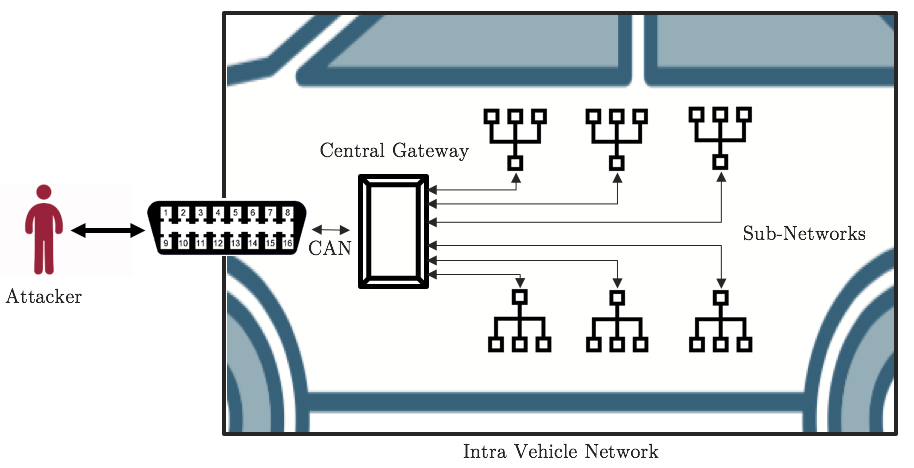
\includegraphics[width=\textwidth]{attackmodel_1.png}
	\caption{Attacker with physical access.}
\end{figure}

\begin{figure}[h]
	\label{fig:attackmodel_2}
	\centering
	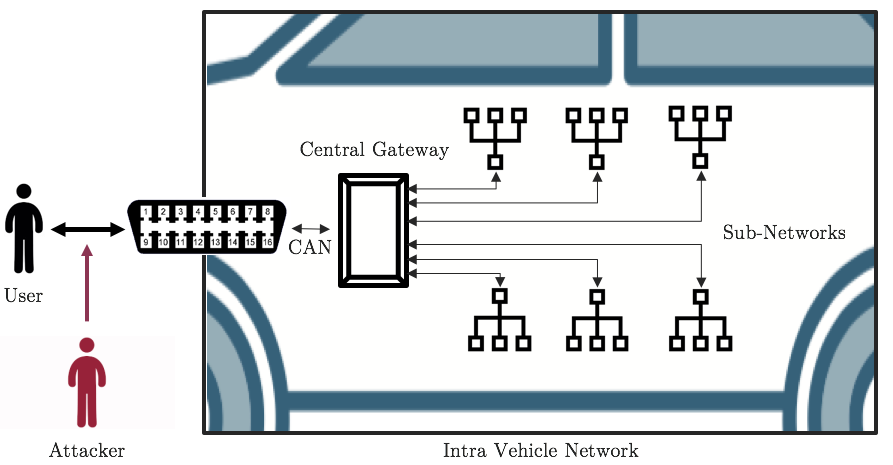
\includegraphics[width=\textwidth]{attackmodel_2.png}
	\caption{Attacker hijacking another OBD-II session.}
\end{figure}

\subsection{Type of Attacker}
Aside from the type of attacks that are possible, it is valuable to define which type of attackers would be interested in attempting them and why. The European Union Agency for Network and Information Security (ENISA) defines 4 types of cyberattacks on smart cars in \cite{Enisa}: 

\begin{itemize}
	\item \textbf{Attacks targeting driver/passenger safety:} This is probably the most serious and harmful type of attacks, since they directly involve the safety of the passengers. Why anyone would be motivated to jeopardize the well-being of another person can vary: extortion, financial gain, rivalries, etc. In the context of OBD-II it is the second attack scenario (i.e. remote OBD-II session hijacking) that is especially relevant here, since these would allow an adversary to initiate the attack while the vehicle is on the road. However, it is not entirely unlikely that someone would compromise the vehicle via the OBD-II interface beforehand, with the intention of compromising drivers/passenger in the future.
	
	\item \textbf{Persistent vehicle alteration by legitimate users:} Most car owners will never concern themselves with the OBD-II interface, and might not even know it exists. Others however, albeit out of sheer curiosity, might take an interest and discover all the possibilities that the OBD-II has to offer. These 'automotive network adventurers' could inadvertently compromise the integrity of the network, thereby endangering themselves and all their passengers. Another incentive for people to alter the behaviour of their own vehicle is personal gain: lowering the internal odometer value before selling the vehicle, clearing recent crash data to fool insurance companies, recalibrating sensors to pass emissions tests, improving the performance of the engine, etc.  
	
	\item \textbf{Surveillance:} The DLC connectors with wifi/Bluetooth capabilities presented in Section \ref{subsec:obd:pid} enable adversaries to remotely monitor the position of the vehicle, and by extension the driver and passengers. This could be taken even further if the GPS system could be remotely compromised. There are many reasons why an adversary or an organisation would be interested in collecting vehicle locations; depending on the type of surveillance: 
	\begin{itemize}
		\item \textbf{Targeted Surveillance:} Where tracking is facilitated by exploiting a vulnerability of a specific individual's vehicle. The effort and cost involved in such an operation hints at the following motives: espionage, crime, terrorism, or business intelligence.
		
		\item \textbf{Mass surveillance:} where a great number of individuals are tracked by exploiting some common vulnerability. Because of the scope these types of attacks, it is likely they are issued by government agencies and criminal organisations.
	\end{itemize}
	
	
	\item \textbf{Theft:} While exploiting remote keyless entry (RKE) vulnerabilities (see Section \ref{subsubsec:rke}) and replaying Radio Frequency identification (RFID) signals (see Section \ref{subsubsec:rfid}) are more common ways of stealing cars, it is not entirely unlikely for the OBD-II interface to be exploited as well. For example, a resourceful adversary could inject a series of messages via the OBD-II interface; tricking the vehicle into starting the ignition.	
\end{itemize}

To sum up, our solution should defend against two different attack scenarios: direct physical access and remote session hijacking. Additionally, we must not underestimate the resources and capabilities of potential attackers. Since, they could range from an inquisitive vehicle owner, to an entire company or government agency. Also, the impact of these attacks can vary from essentially harmless, to physically endangering drivers and their passengers; indicating that care must be taken to design a system that is sufficiently secure. To further illustrate the security vulnerabilities of OBD-II, a series of example attacks are presented in the next section.

\subsection{Example attacks}
\label{subsec:example_attacks}

The exploits that are presented here were performed by Charlie Miller and Chris Valasek and documented in \cite{MillerC}; in an effort to raise awareness about the issue, as well as allowing car manufacturers to build safer cars in the future. They accomplished this by not only finding and exploiting various vulnerabilities in extant vehicles, but also sharing any software that made these exploits possible. An example of this is EcomCat, which is software written to aid in the reading and writing of data to the CAN bus through one or more Ecom cables \cite{MillerC}. The Ecom cable is then used to connect a laptop to the OBD-II DLC; allowing the researchers to use their EcomCat software to inject their own CAN messages onto the internal bus. Although seemingly straightforward, there are many potential problems in attempting to make the vehicle perform actions by injecting packets on the CAN bus. First, not everything can be controlled via the CAN bus (e.g. cruise control). Second, if a specific type of CAN packet is found to be a request (An ECU asking for another ECU to perform an action), replaying a fake copy does not guarantee that the message is accepted. This is because the original message is still sent; possibly confusing the ECU with conflicting information. Third, It is also possible that fake messages are ignored because of built-in security features inside the ECU. Despite these difficulties, these researchers did manage to mount a series of interesting exploits, three of which are presented here next.

\subsubsection{Speedometer} 
\label{subsubsec:speedometer}

In this example, performed on a 2010 Toyota Prius, the researchers managed to identify the messages that are sent to the speedometer to display the current velocity of the vehicle. Replaying this message with custom data fields allowed them to display any arbitrary speed on the speedometer display.

\subsubsection{Denial of Service} 
\label{subsubsec:denial_of_service}

Here the researches cleverly take advantage of how the CAN protocol works. Remember from section \ref{subsec:can:message_arbitration} that CAN uses priority scheduling over the ID's of the messages that are sent on the bus. This means that spamming a high priority message would prevent all other messages from being transmitted. This vulnerability is exploited here by flooding the bus with CAN messages with an ID of 0. This flooding of the CAN bus halts the engine from being turned on, as well as putting the system in an all out state of disarray.

\subsubsection{Diagnostic session} 
\label{subsubsec:diagnostic_session}

The aforementioned examples used injection of messages that are normally sent from ECU to ECU, thereby erroneously invoking certain actions. Another approach is to trick the vehicle network into starting a diagnostic session; these are used in normal circumstances by a technician at a garage. It allows them to test the function of an ECU without having to take the vehicle on the road, as well as recalibrating them. Starting a diagnostic session does require circumventing an authentication procedure (see \ref{sec:obd_access_control}); however, this proved rather easy (this was done by reverse engineering an official authentication device and extracting the keys). Once a diagnostic session was established it opened up a wide array of possible attacks: Killing the engine, disabling the brakes, honking the horn, unlocking/locking doors, and even reprogramming of certain ECU's (see \cite{MillerC} for a detailed description of the attacks).

\section{Ideal OBD-II System}
\label{sec:sol_RBAC}

They key research question here is: can a solution be developed that would protect an in-vehicle network from unauthorised access via the OBD-II port. The concept of 'unauthorised access' is key, since the goal is not to deny access altogether. Only authorised personnel (e.g. repairmen) should be allowed high levels of access; only they should be allowed to start diagnostic sessions, recalibrate ECU's, etc. The only way of differentiating between what is allowed and what is not, is by looking at the messages that are sent, specifically their ID's. Some messages, like a message asking for the status of a certain ECU, could be considered harmless. The message that is used to initiate a diagnostics session however is not that innocent, since it is shown in \cite{MillerC} that this could be used to disengage the brakes, kill the engine, etc. It follows that any solution to this problem should involve a series of authorisation levels, and that each one of these roles should associated with a number of permitted message ID's. The concept of role-based access control presented in Section \ref{sec:RBAC} is clearly applicable here. \\ \\ The next question to answer is where this system of access control should enforced. The assertion made in Section \ref{sec:motivation}, stating that the main problem of OBD-II is the indiscriminate nature at which the gateway forwards messages coming from the interface, hints at the ideal solution. Because of it's strategic position and privileged role in forwarding messages, the gateway is the ideal location to enforce a RBAC system for OBD-II. Another reason for this is the fact that our solution should be software based, as is discussed in Section \ref{sec:challenges}. A solution that requires the introduction of dedicated hardware, would result in a system that is difficult to implement in practice. Indeed, it would require significant cost and effort from car manufacturers to modify the hardware of millions of currently in-use vehicles. A software update of extant gateway ECU's on the other hand, requires significantly less effort. \\ \\ The final question is how to enforce RBAC in practice. In a common enterprise RBAC system, the worker authenticates to the system via some type of authentication key. this key can be literally: physical key, key-card, software key, etc. However, in some instances this key is represented by some type of secret knowledge (like a password or PIN-code) or even some identifying characteristic of the individual (fingerprint scan, retinal scan, etc). The  worker authenticates to the system by proving (s)he is in possession of the appropriate key. Translating this concept to our situation; the user (e.g. car owner, repairman, policeman, etc) authenticates to the system (the gateway of the vehicle) by proving that (s)he in possession of the appropriate key. The system will verify this key before granting the permissions that correspond to the appropriate role. It should come as no surprise that an authentication scheme based on software keys is appropriate here. \\ \\ Every authorisation level constitutes a role, and what messages are allowed for each level constitute the permissions of this role. More specifically, this system should be considered an instance of mandatory access control (see section \ref{sec:RBAC}), since the users are not allowed any control over what permissions they are granted. Now that a system of access control is introduced, we need to look at how this system can be implemented to protect the OBD-II port.

\section{OBD-II Access Control}
\label{sec:obd2_access_control}

It's time to present our solution. Our proposal constitutes a RBAC system for the OBD-II interface, that employs asymmetric key pairs to authenticate users. This system is illustrated in Figure \ref{fig:solution}. The choice was made to make use of cryptographic keys to implement access control. This means that users will have to prove they are in possession of the appropriate cryptographic key, in order for them to gain access to the vehicle network. Introducing a single cryptographic key that grants access to all extant vehicles is considered infeasible (requiring all vehicle manufacturers to cooperate), as well as insecure (disclosure of this single key would result in the exposure of all vehicles). This is why we propose to introduce different cryptographic keys for every vehicle model. From Section \ref{sec:PKC} it follows that there are two distinct cryptographic key technologies that can be considered: symmetric and asymmetric. Symmetric cryptography has the advantage of shorter key lengths and faster calculations, however this would entail that if the keys of one vehicle were extracted and distributed (e.g. by physically analysing the gateway), all vehicles of the same model would be compromised. That is why the decision was made to use asymmetric keys for authentication, as well as generating a temporary symmetric key. This symmetric key can then be used to secure the following communications session against session hijacking. \\ \\ The gateway stores a series of public keys, each one associated with a specific role. A user wishing to authenticate him/herself would have to prove the ownership of the appropriate private key.\footnote{This key ownership configuration could be flipped (i.e. gateway stores private key and user owns public key). However, this configuration has the same major design flaw that symmetric encryption had, namely possible extraction of the private key from the vehicle} The decision to use asymmetric keys moves the responsibility of safely storing the private key to the users. Intuitively this might seem like a bad idea, since now the private keys are already in the hands of individuals; individuals that might have ulterior motives concerning their level of access. This flaw was countered by introducing a central server that safely stores the private keys, together with an internet connected device called a tester that physically connects to the OBD-II port. Users with privileged roles will first authenticate to the central server via the tester, using some other authentication method (e.g. login and password). This dedicated device will then initiate an authentication procedure with the gateway, proving ownership of the appropriate private key while also establishing a shared secret. This authenticated key agreement procedure is discussed in more detail next.

\begin{figure}[h]
	\label{fig:solution}
	\centering
	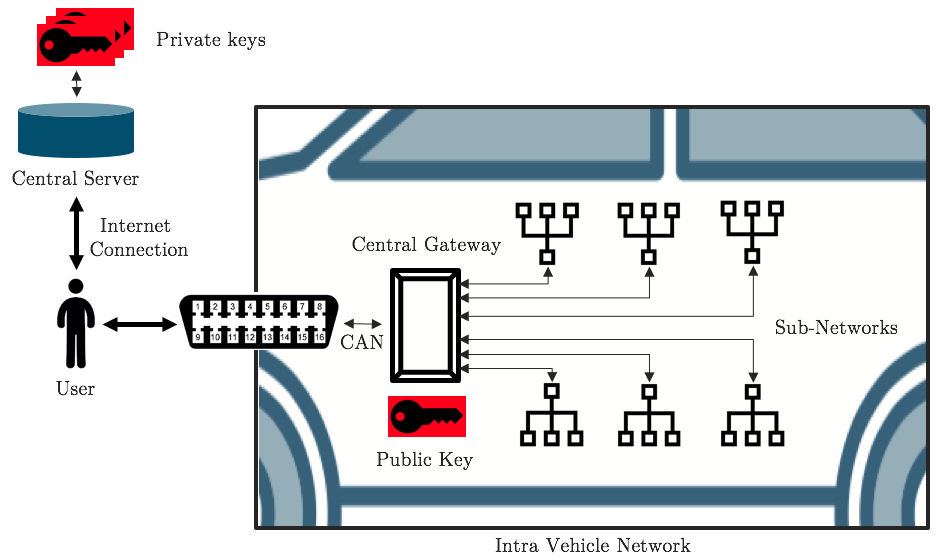
\includegraphics[width=\textwidth]{solution.png}
	\caption{OBD-II access control architecture.}
\end{figure}


\subsection{Authenticated Key Agreement Procedure}
\label{subsec:authenticated_key_agreement_procedure}

The goal of the authenticated key agreement procedure is to prove to the gateway that the user is in possession of the appropriate private key, while also initiating an authenticated session between tester and gateway by calculating a shared secret key. This calculation would incorporate the pre-shared asymmetric keys, thereby combining authentication and secret key establishment into a single procedure. This procedure is based on the ECDHE\_ECDSA algorithm introduced in Section \ref{subsubsec:ecdh_ecdsa}, specifically Figure \ref{fig:ECDH2}. A couple of changes were applied to this algorithm to more closely adhere to our situation:
\begin{enumerate}
	\item \textbf{Gateway Key Pair:} A precondition for the ECDHE\_ECDSA algorithm is that both parties have an ECC key pair already established. For the tester this condition is already met; even better, the corresponding public key is already given to the gateway. However, for the gateway this is not the case. ECDH requires two key pairs, so a new key pair will have to be computed every time the procedure is run.
	
	\item \textbf{Perfect Forward Secrecy:} We can get rid of the ephemeral keys. This is because perfect forward secrecy (or secrecy in general) is not a goal in our situation. the goal is to protect against unauthorised access, not to protect past sessions from leaking. 
	
	\item \textbf{Mutual Authentication:} The first authentication step can be omitted (i.e signing by the gateway, and verification by the tester). Because of the absence of a gateway key pair, it is impossible for the gateway to authenticate itself to the tester. Moreover, this is not even a requirement of our authentication procedure.
\end{enumerate}
Considering these modifications, the procedure from Figure \ref{fig:authentication_procedure} is obtained. Before the procedure is initiated, the central server is in possession of the OBD-II private key $Pr_{obd}$, while the gateway has the appropriate public key $Pb_{obd}$ stored in memory. The user of the tester initiates the procedure by connecting to the OBD-II port, after which the tester sends an initialization message to the gateway. This initialization message also specifies the role that the user of the tester wishes to authenticate as. The gateway responds to this by creating a new ECC key pair: KGen($Pb_g$,$Pr_g$), and sending the newly created public key $Pb_g$ to the tester. The tester then forwards this secret key to the central server, which in turn signs this public key using the OBD-II private key: Sig($Pb_g$,$Pr_{obd}$), before sending the signature back to the tester. The tester then forwards this signature (only the signature) back to the gateway. After the gateway has verified the signature using the OBD-II private key: Ver(Sig,$Pb_{obd}$), both parties calculate the shared secret using ECDH. The gateway does this by calculating $K$=ECDH($Pr_g$,$Pb_{obd}$). The tester however does not have all the ingredients to do so, since the OBD private key is stored on the central server. That is why the shared secret is generated on the server, before being securely transmitted to the tester. This newly created secret can then be used by both communicating parties to authenticate every OBD-II message that is sent in the upcoming session; this procedure is discussed next.
 
\begin{figure}[h]
	\centering
	\fbox{
		\procedure{OBD-II authenticated key agreement procedure}{%
			\textbf{Central Server} \<\< \textbf{Tester}  \<\< \textbf{Gateway} \\
			\text{$Pr_{obd}$} \<\<\<\< \text{$Pb_{obd}$} \\
			\<\< \< \sendmessageright{length=1.5cm,top=\text{init}} \<\\
			\<\<\<\< \text{KGen($Pb_g$,$Pr_g$)} \\
			\<\sendmessageleft{length=1.5cm,top=\text{$Pb_g$}} \<\< \sendmessageleft{length=1.5cm,top=\text{$Pb_g$}} \<\\
			\text{$S$=Sig($Pb_g$,$Pr_{obd}$)} \<\<\<\< \\
			\< \sendmessageright{length=1.5cm,top=\text{$S$}} \<\< \sendmessageright{length=1.5cm,top=\text{$S$}} \<\\
			\<\<\<\< \text{Ver($S$,$Pb_{obd}$)} \\
			\text{$K$=ECDH($Pr_{obd}$,$Pb_g$)} \< \sendmessageright{length=1.5cm,top=\text{$K$}} \<\<\< \text{$K$=ECDH($Pr_g$,$Pb_{obd}$)} \\
		}
	}
	\caption{OBD-II authenticated key agreement procedure}
	\label{fig:authentication_procedure}
\end{figure}

\subsection{Message Authentication Procedure}
\label{subsec:message_authentication_procedure}

The authentication procedure from Section \ref{subsec:authenticated_key_agreement_procedure} authenticates the tester to the gateway, thereby also establishing a shared secret. The next step is to design a procedure that uses this shared secret to facilitate an authenticated communications session. The solution proposed by the researchers of this paper is simple, and is illustrated in Figure \ref{fig:message_authentication}. The OBD-II message $M$ sent by the tester is followed up by a message containing a MAC: MAC($M$,$K$) (see Section \ref{subsec:MAC}). This MAC is calculated by inputting the data of the first CAN frame as well as the recently established secret key $K$. Before the gateway forwards the message to the appropriate sub-network, it first performs two distinct security checks: 
\begin{itemize}
	\item \textbf{Permissions Check CheckP($M$):} This is where the role based access control system proposed in Section \ref{sec:sol_RBAC} is actually enforced. The user specified his/her role in the initialization message, so the gateway knows the role of the user. The first condition that is checked is whether this role has permission to send the message $M$. It will do this by looking up the ID of the message in the permissions table (see Section \ref{sec:permissions_table}). If the role does not have the permission to send the message, it will be denied and the tester (and by extension the user) is notified.
	
	\item \textbf{MAC Verification Ver(MAC,$K$):} After the message $M$ passes the permissions check, the gateway will check whether the received MAC is correct; ensuring that the sender of this message is authorized. Again, if this test fails the message will be denied and the tester is notified
\end{itemize}
If both these checks succeed, the OBD-II message $M$ is forwarded to the appropriate sub-network and the tester receives an acknowledgement (ACK). 

\begin{figure}[h]
	\centering
	\fbox{
		\procedure{OBD-II message authentication procedure}{%
			\textbf{Tester}  \<\< \textbf{Gateway} \<\< \textbf{Network}\\
			\text{$K$}  \<\< \text{$K$} \<\< \\
			\< \sendmessageright{length=3cm, top=\text{OBD-II message $M$}} \<\<\<\\
			\<\< \text{CheckP($M$)} \<\< \\
			\< \sendmessageright{length=3cm, top=\text{MAC($M$,$K$)}} \<\<\<\\
			\<\< \text{Ver(MAC,$K$)} \<\< \\
			\<\<\< \sendmessageright{length=3cm, top=\text{$M$}} \< \\
			\< \sendmessageleft{length=3cm, top=\text{ACK}} \<\<\< \\
		}
	}
	\caption{OBD-II message authentication procedure}
	\label{fig:message_authentication}
\end{figure}

\subsection{Permission Table} 
\label{subsec:sol_permissions_table}
The permission table is stored on the gateway, and is used to determine which OBD-II messages are allowed for each role. Before looking at the design of the OBD-II permission table, we need to concretely define the roles themselves. It is worth noting that the selection made here is purely for demonstrative purposes. Significant additional research would have to be conducted to determine what roles are necessary for this system to adhere to the current automotive landscape. This topic is discussed in more detail in Section \ref{sec:future_research}.

\begin{itemize}
	\item \textbf{Admin:} This role is not related to the intra vehicle network, but rather the OBD-II access control system itself. It is essential that the software that enforces RBAC on the gateway can be updated and configured. Any user authenticating themselves as an admin will have the ability to send specific control messages that are designed to modify the existing RBAC software on the gateway. Which includes adding and removing roles, replacing public keys when the corresponding private key was compromised, apply patches that are designed to fix bugs, etc.
	
	\item \textbf{OEM:} The original equipment manufacturer (OEM) refers to the company that designed and produced the various ECU's that are found inside the vehicle. By extension, the manufacturer of the vehicle itself is considered an OEM. Workers authenticating themselves as an OEM need considerable control over the intra vehicle network to correctly test, configure and update ECU's. This is why this role will generally be granted a high level of clearance.
	
	\item \textbf{Repairman:} Probably the most obvious candidate for a role since OBD-II was designed first-and-foremost to diagnose and fix vehicle malfunctions. And this is exactly what repairmen are employed to do.
	
	\item \textbf{Policeman:} In Section \ref{subsec:informal_model} we discussed the possibility of car owners illegally tampering with their own vehicles (e.g. reducing odometer values before selling). It is up to law enforcement to prohibit this kind of behaviour, and the most efficient way of doing so is by interfacing with the OBD-II interface. This is why policemen should be granted their own role; allowing them to check ECU's that are frequently the subject of tampering.
	
	\item \textbf{Owner:} This role corresponds to the lowest level of clearance. The owner of the vehicle is only trusted with harmless OBD-II messages; allowing adventurous vehicle owners to safely interact with their vehicle's intra vehicle network.
\end{itemize}
The general architecture of RBAC permission tables is as follows: every entry in the table is associated with a permission, or in this context, the ID of a specific CAN message. Each entry will have series of fields (equal to the amount of roles that are defined), and each field signals whether the corresponding permission is granted to the role of that particular field. Table \ref{table:2} shows the design of the table. A value of 1 means the corresponding role has the permission to send a message with the corresponding ID. This design includes three examples taken from \cite{MillerC}, which are CAN messages that are transmitted in the intra vehicle network of a 2010 Ford Escape. The message with IDH: 02 and IDL 01\footnote{Remember from Section \ref{subsec:can:frames} that a base format CAN has an ID of 11 bits. In CAN controllers this ID is often split up into two hexadecimal values IDL and IDH, where IDL equals the eight least significant bits, and IDH equals the three most significant bits.} is used to display the current speed and rounds per minute. The message with IDH: 04 and IDL: 02 is used to update the value of the internal odometer. And, the message with IDH: 00 and IDL: 00 is not used to indicate a specific function, but could be used to mount a denial of service attack. These examples indicate how a security policy can be established via the permission table. For example, every role has the permission to send the speedometer message (IDH: 02, IDL 01), since it could be considered harmless. The odometer message (IDH: 04, IDL: 02) is rejected for both the Owner and Repairman roles, since they are most likely to tamper with it. And, the highest priority message (IDH: 00, IDL: 00) is only allowed for the Admin and OEM roles.

\begin{table}[]
	\begin{tabular}{|c|c|c|c|c|c|}
		\hline
		\rowcolor[HTML]{9B9B9B} ID & Admin & OEM & Repairman & Policeman & Owner \\ \hline
		\cellcolor[HTML]{9B9B9B} IDH: 02, IDL: 01 & 1 & 1 & 1 & 1 & 1 \\ \hline
		\cellcolor[HTML]{9B9B9B} IDH: 04, IDL: 02 & 1 & 1 & 0 & 1 & 0 \\ \hline
		\cellcolor[HTML]{9B9B9B} IDH: 00, IDL: 00 & 1 & 1 & 0 & 0 & 0 \\ \hline
		\cellcolor[HTML]{9B9B9B} \vdots & \vdots & \vdots & \vdots & \vdots & \vdots
	\end{tabular}
	\caption{OBD-II permissions table design \& example.}
	\label{table:2}
\end{table}



\paragraph{}
To sum up, our proposal employs cryptographic keys to apply a RBAC model to the OBD-II system. More specifically, an asymmetric key pair is associated with every role. The corresponding private key is distributed to the appropriate users (e.g. manufacturers, repairmen, policemen, etc), while the public keys are stored on the vehicle gateway. Whenever a user wishes to gain access to the intra vehicle network via the OBD-II port, (s)he will first have to authenticate him/herself by proving (s)he is in possession of the appropriate private key. This is done by completing an authenticated key agreement procedure, whereby the user is authenticated and a temporary symmetric key is established. Next, a message authentication procedure is performed for every message that is sent by the user. This procedure uses the aforementioned temporary symmetric key to authenticate every message. On top of checking the authenticity, the permission table is checked as well for every message. This permission table determines which messages are allowed for each role, effectively determining the security policy of the OBD-II RBAC system.





\chapter{Implementation and Evaluation}
\label{chap:implementation}

In Section \ref{sec:challenges} we presented the three main challenges of this research paper: portability, speed and security. To accurately assess whether the design presented in Chapter \ref{chap:solution} meets these challenges, an example system was implemented by the researchers of this paper. The first part of chapter is devoted to illustrating the various aspects of this implementation. In the second part of this chapter, this implementation is evaluated and analysed with regard to the challenges proposed earlier. 

\section{Implementation}
\label{sec:implementation}

The structure of this section is as follows: First, the individual pieces of hardware that were used in the implementation are discussed. Second, the set-up of the demo in general is explained. In the last section of this chapter, the implementations of the three key aspects of Section \ref{sec:obd2_access_control} are illustrated (authenticated key agreement procedure, message authentication procedure and permissions table).

\subsection{Hardware}
\label{sec:hardware}
It is clear that the design presented in Chapter \ref{chap:solution}, as well as the OBD-II system is general, is of an embedded nature. The gateway ECU is embedded by default, since it is implemented by a microcontroller in all extant intra vehicle networks. The tester device however, introduced by the researchers of this paper, could be either implemented by an embedded device (e.g. tester), or a software application running on a standard PC (e.g. a laptop owned by the repair shop), that is connected to the OBD-II port via some adapter. The decision was made to implement the former (i.e. the tester is also embedded). Because of this decision, the tester and gateway can be implemented on the same microcontroller architecture. This also means that the same CAN messaging library can be used in both microcontrollers.\\ \\ The goal of this implementation is to serve as a proof of the practical feasibility of our proposed solution. This is why the choice of hardware architecture is very important. The idea is that if an implementation on a resource constrained microcontroller, would meet our challenges (i.e. portability, security and speed); This would prove that implementation is possible on all microcontrollers that feature better specifications than the one we used in our demo. This is why we chose to select a microcontroller architecture that is as limited as possible.  \\ \\ The microcontroller chosen for our implementation is the Atmel AT90CAN128. Which has a word size of 8 bits, boasts a 128 KB flash memory, 4KB of EEPROM and 4KB SRAM (for more information on these specifications see  Section \ref{sec:microcontrollers}). The CPU of this microcontroller was run at a clock speed of 8 MHz. More importantly, it includes a dedicated CAN controller, which allows for easy CAN networking between devices. The DVK90CAN1 is a development kit that includes the AT90CAN128, as well as introducing a series of hardware peripherals like power supply inputs, LEDS, buttons, connectors, transceivers, programming interfaces, debuggers, etc. The ones that were extensively used in our implementation are:
\begin{itemize}
	\item \textbf{Programming/Debugging interface:} The DVK90CAN1 includes the option of easily connecting to a standard PC for programming and debugging. This is done by connecting the ATMEL-ICE BASIC programmer to both the DVK90CAN1 board and a PC running Atmel Studio, which is an integrated development platform (IDP) that allows us to run and debug C and assembly code on both microcontrollers.
	
	\item \textbf{CAN transceiver:} This device functions as a transmitter and receiver by transmitting messages from the CAN controller on to the CAN bus (male DB9), as well as receiving incoming CAN messages and forwarding them to the CAN controller; effectively implementing the physical layer of CAN.
	
	\item \textbf{Male DB9 connector:} This connector belongs to the D-sub series, where the B denotes the shell size and the 9 means there are 9 pins. This connector assumes the CAN bus connections.
	
	\item \textbf{RS-232 driver/receiver:} Recommended standard 232 (RS-232) is a standard for serial transmission of data. The driver/receiver is responsible for transmitting and receiving RS-232 data (female DB-9).
	
	\item \textbf{Female DB9 connector:} This connector assumes the RS-232 connections.
	
	\item \textbf{Compass Card Keyboard} 4 de-centered push-buttons of compass card keyboard are present on the board, allowing for user interactivity.
\end{itemize}
Besides some peripherals offered by the DVK90CAN1 board and the ATMEL-ICE BASIC programmer, two more pieces of hardware were use in our system. First, there's a female-to-female DB9 cable. This is used to connect the CAN interfaces of both boards. Second there's a male-to-male DB9 cable that is connected to a generic RS232 to USB converter. This cable allows both boards to be connected to a PC for serial communications.

\subsection{Demo Set-Up}
\label{sec:demo_setup}

Figure \ref{fig:demo} shows the set-up of our implementation. One board functions as the tester (the one on the left), which is connected via CAN (using the female-to-female DB9 cable) to the other board (the one in the middle), which in turn functions as the gateway. This connection is used to implement the general authenticated key agreement and message authentication procedures presented in Section \ref{subsec:authenticated_key_agreement_procedure} and \ref{subsec:message_authentication_procedure}. The permission table outlined in Section \ref{subsec:sol_permissions_table} is implemented on the gateway. The gateway is also connected to a PC using the RS-232 communications standard, to allow for real time feedback (e.g. signalling when a signature verification procedure successfully terminates). The attentive reader might notice two integral components missing from this set-up: the central server that is introduced in Section \ref{fig:authentication_procedure}, as well as the intra vehicle network itself. The decision was made to implement these components only logically. This was done for two reasons: first, a realistic implementation of these components would result in the introduction of more hardware, greatly increasing the time and cost required to construct a working demo. Second, since the primary focus of this paper is the RBAC system proposed in Chapter \ref{chap:solution}, as well as all the procedures and systems introduced to enforce it on the gateway (i.e. authenticated key agreement procedure, message authentication procedure and permissions table); providing a physical central server and intra vehicle network implementation can be considered out of scope. The logical implementation of both these components was done as follows:
\begin{itemize}
	\item \textbf{Central Server:} The software on the tester board implements a dedicated key-API that specifies a series of private key related functions (for signing and calculating the shared secret). As far as the main tester software is concerned, calling these functions could result in a remote server being addressed.
	
	\item \textbf{Intra Vehicle Network:} The RS-232 connection between gateway and PC is used for this purpose. Whenever a message is accepted by the gateway, instead of forwarding the message to another sub-network, a message is transmitted to the PC. This message contains the ID of the accepted message, as well as a line of text signalling that the message was accepted.
\end{itemize}

\begin{figure}[h]
	\centering
	\includegraphics[width=\textwidth]{demo_setup.jpg}
	\caption{Hardware set-up that is used to implement the proposed solution.}
	\label{fig:demo}
\end{figure}

\subsection{OBD-II Access Control Implementation}
The key aspects aspects of the OBD-II access control system presented in Chapter \ref{chap:solution} are the authenticated key agreement procedure, the message authentication procedure and of course the permissions table. How these were implemented in the set-up presented in Section \ref{sec:demo_setup} is discussed next. The source code of our implementation can be found in \cite{Michel}.  

\subsubsection{Authenticated Key Agreement Procedure Implementation}
\label{subsec:authenticated_key_agreement_procedure_implementation}

Figure \ref{fig:authentication_procedure_implementation} shows how the authentication procedure was implemented in our demo. Because of our decision to omit the central server and the intra vehicle network, these are naturally not included in the diagram. Because of this, the tester now stores the OBD-II private key $P_{obd}$ instead of the central server. In our diagram we have chosen to include the size of this key (in bits) in the superscript: $Pr_{obd}^{256}$. This was repeated for every piece of data in the diagram (e.g. keys and signatures). The corresponding public key $Pb_{obd}^{512}$ is stored on the gateway. The size of these keys was mandated by the decision to guarantee a security level of 128 bits (see Section \ref{sec:security_level}). As mentioned in Section \ref{subsec:ECC}, the decision was made to use elliptic curve asymmetric key pairs. The TinyECC\footnote{\url{https://github.com/kmackay/micro-ecc}} C library offers a safe and efficient implementation for ECC operations on AVR microcontrollers. According to \cite{Siddiqui}, ECC keys have the property that the size of the underlying field (i.e. the size of the private key), should be twice the security parameter \cite{Siddiqui}. The decision was made to work with the secp256r1 curve (also supported by TinyECC), which meets our security level guarantee ($\frac{256}{2}=128$) and introduces fixed sizes for our keys (256 bit for the private key and 512 bits for the public key).

\paragraph{The Procedure}

The authentication procedure is initiated by the tester, which transmits an initialisation message to the gateway. This message contains the role that the tester wishes to authenticate as: $Role^8$. Because it is only 8 bits in size, it fits into a single CAN message (remember from Section \ref{subsec:can:frames}, that a CAN message can hold up to 64 bits of data). The gateway reacts to this message by creating a new ECC keypair: KGen($Pb_g^{512}$,$Pr_g^{256}$. The same curve must be used as the one chosen for the original OBD-II keys (i.e. secp256r1), otherwise the ECDH secret generation algorithm used later on will not work. As a result of this, both key pairs have the same respective sizes. Next, the newly generated public key $Pb_g^{512}$ is transmitted to the tester. Because of it's size (512 bits), this key won't fit into a single CAN message. This problem is overcome by spreading the key over 8 distinct CAN messages, and sending them to the tester one by one. After the tester has received all 8 messages, and has assembled the public key, it will first hash it using SHA512: SHA512($Pb_g^{512}$). For this operation the AVR cryptolib\footnote{\url{https://github.com/cantora/avr-crypto-lib}} C library was chosen. After calculating the hash value, the signing function of the key API is called: Sig(SHA512($Pb_g^{512}$),$Pr_{obd}^{256}$). This results in the signature being generated: $S^{512}$. The size of our signature is determined by our choice of curve; our curve corresponds to a signature size of 512 bits. Once the signature is generated, it sent to the gateway. Because the signature is the same size as the public key that was sent earlier, it is also spread over 8 different CAN messages. Upon reception, the gateway verifies the validity of the signature by first hashing it with the same hash function used in its generation (SHA512), before running the ECDSA verification procedure: Ver(SHA512($S^{512}$),$Pb_{obd}^{512}$). If and when the verification is successful, an ACK message is transmitted to the tester. Both tester and gateway can now generate the shared secret: ECDH($Pr_{obd}^{256}$,$Pb_g^{512}$) and ECDH($Pr_g^{256}$,$Pb_{obd}^{512}$), which will be used in the message authentication procedure.

\begin{figure}[h]
	\centering
	\fbox{
		\procedure{OBD-II authenticated key agreement procedure implementation}{%
			\textbf{Tester}  \<\< \textbf{Gateway} \\
			\text{$Pr_{obd}^{256}$} \<\< \text{$Pb_{obd}^{512}$} \\
			\< \sendmessageright{top=\text{$Role^8$}} \<\\
			\<\< \text{KGen($Pb_g^{512}$,$Pr_g^{256}$)} \\
			\< \sendmessageleft{top=\text{$Pb_g^{512}$}} \<\\
			\text{$S^{512}$=Sig(SHA512($Pb_g^{512}$),$Pr_{obd}^{256}$)} \<\<\<\< \\
			\< \sendmessageright{top=\text{$S^{512}$}} \<\\
			\<\< \text{Ver(SHA512($S^{512}$),$Pb_{obd}^{512}$)} \\
			\< \sendmessageleft{top=\text{$ACK^{8}$}} \<\\
			\text{$K^{256}$=ECDH($Pr_{obd}^{256}$,$Pb_g^{512}$)} \<\< \text{$K^{256}$=ECDH($Pr_g^{256}$,$Pb_{obd}^{512}$)} \\
		}
	}
	\caption{OBD-II authenticated key agreement procedure implementation.}
	\label{fig:authentication_procedure_implementation}
\end{figure}



\subsubsection{Message Authentication Procedure Implementation}
\label{subsec:message_authentication_procedure_implementation}

Figure \ref{fig:message_authentication_implementation} shows the implementation of the message authentication procedure. After the procedure from Section \ref{subsec:authenticated_key_agreement_procedure_implementation} completes, and the shared secret $K$ is established, this procedure is repeated for every OBD-II message sent by the tester. The procedure starts when the tester sends the message $M^{64}$ (again superscript is used to indicate the size). The gateway receives the message and checks the permissions table: CheckP($M^{64}$) (see Section \ref{subsec:permissions_table_implementation}), before sending an acknowledgement back to the tester: $ACK^8$. This acknowledgement is positive or negative based on the outcome of the earlier permissions table check. Upon reception of the acknowledgement, the tester calculates the MAC of the message using the shared secret and HMAC\textunderscore SHA256: $Mac^{256}$=Hmac\textunderscore SHA256($M$,$K$). For the HMAC\textunderscore SHA256 operation the AVR cryptolib library is used, just like we did for SHA512 in Section \ref{subsec:authenticated_key_agreement_procedure_implementation}. The size of this MAC is again mandated by our security guarantee of 128 bits. This is because the SHA265 cryptographic hash algorithm has a security level of 128 bits against collision attacks \cite{SHA256Collision}. The MAC is then sent to the Gateway, which will in turn verify it using the shared secret: Ver($Mac^{256}$,$K$). If the MAC is valid, the original message $M^{64}$ is forwarded to the intra vehicle network: Forward($M^{64}$), which in our implementation was indicated by sending a RS232 message to a connected PC. The tester is also informed of this by sending another acknowledgement. Upon reception the tester might want to send another message, in which case the entire procedure is repeated. 

\begin{figure}[h]
	\centering
	\fbox{
		\procedure{Message Authentication Procedure Implementation}{%
			\textbf{Tester}  \<\< \textbf{Gateway} \\
			\text{$K$}  \<\< \text{$K$} \\
			\< \sendmessageright{top=\text{OBD-II message $M^{64}$}} \<\\
			\<\< \text{CheckP($M^{256}$)} \\
			\< \sendmessageleft{top=\text{$ACK^8$}} \< \\
			\text{$Mac^{256}$=Hmac\textunderscore SHA256($M$,$K$) } \<\< \\
			\< \sendmessageright{top=\text{$Mac^{256}$}} \<\\
			\<\< \text{Ver($Mac^{256}$,$K$)}  \\
			\<\< \text{Forward($M^{64}$)}  \\
			\< \sendmessageleft{top=\text{$ACK^8$}} \< \\
		}
	}
	\caption{OBD-II Message Authentication Implementation}
	\label{fig:message_authentication_implementation}
\end{figure}

\subsubsection{Permission Table Implementation}
\label{subsec:permissions_table_implementation}

The permission table is implemented according to the design of Section \ref{subsec:permissions_table}. Generally, a permission table for a RBAC system will use hash functions to map user names to fixed size indices. However, in our case the user names are replaced by CAN message ID's, which already have a fixed size of 11 bits (or 29 if the extended frame format is used), negating the need for any hash functions. Table \ref{table:roles} lists all the roles currently implemented, as well as their byte representation (This byte representation is also used in the $Role^{8}$ message of the authentication procedure in Section \ref{subsec:authenticated_key_agreement_procedure_implementation}). Table \ref{table:permissions} shows the implementation of the example of Table \ref{table:2} in Section \ref{subsec:permissions_table}. Every ID entry points to a data structure consisting of a series of bytes; each one associated with a role. The presence of a certain role in this series of bytes, indicates that this role has the permission to send a message with the aforementioned ID. Permissions are easily granted and revoked (Admin role) by deleting and adding role bytes to the data structure pointed to by the chosen ID. 

\begin{table}[]
	\centering
	\begin{tabular}{|c|c|c|c|c|}
		\hline
		\rowcolor[HTML]{9B9B9B} 
		Admin & OEM & Policeman & Repairman & Owner \\ \hline
		\rowcolor[HTML]{FFFFFF} 
		00000000 & 00000001 & 00000010 & 00000011 & 00000100 \\ \hline
	\end{tabular}
	\caption{Role implementation}
	\label{table:roles}
\end{table}

\begin{table}[]
	\adjustbox{max width=\textwidth}{%
	\begin{tabular}{|
			>{\columncolor[HTML]{9B9B9B}}c |c|
			>{\columncolor[HTML]{9B9B9B}}c |
			>{\columncolor[HTML]{9B9B9B}}c |
			>{\columncolor[HTML]{9B9B9B}}c 
			>{\columncolor[HTML]{9B9B9B}}c 
			>{\columncolor[HTML]{FFFFFF}}c }
	\hhline{-~-----}
	   IDH: 02, IDL: 01	& 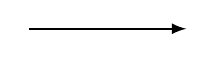
\begin{tikzpicture}[thick] \draw [black,  -latex] (0,6.5) -- (2,6.5); \end{tikzpicture} & 00000000 & 00000001 & \multicolumn{1}{c|}{\cellcolor[HTML]{9B9B9B} 00000010} & \multicolumn{1}{c|}{\cellcolor[HTML]{9B9B9B} 00000011}  & \multicolumn{1}{c|}{\cellcolor[HTML]{9B9B9B} 00000100}  \\ \hhline{-~-----} \multicolumn{1}{c}{\cellcolor[HTML]{FFFFFF}} & \multicolumn{1}{c}{\cellcolor[HTML]{FFFFFF}} & \multicolumn{1}{c}{\cellcolor[HTML]{FFFFFF}} & \multicolumn{1}{c}{\cellcolor[HTML]{FFFFFF}} & \multicolumn{1}{c}{\cellcolor[HTML]{FFFFFF}} & \multicolumn{1}{c}{\cellcolor[HTML]{FFFFFF}} &  \\ \hhline{-~---~~}
	   IDH: 04, IDL: 02	& 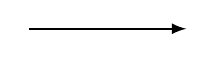
\begin{tikzpicture}[thick] \draw [black,  -latex] (0,6.5) -- (2,6.5); \end{tikzpicture} & 00000000 & 00000001 & \multicolumn{1}{c|}{\cellcolor[HTML]{9B9B9B} 00000011} & \multicolumn{1}{c}{\cellcolor[HTML]{FFFFFF}} &                                               \\ \hhline{-~---~~} \multicolumn{1}{c}{\cellcolor[HTML]{FFFFFF}} & \multicolumn{1}{c}{\cellcolor[HTML]{FFFFFF}} & \multicolumn{1}{c}{\cellcolor[HTML]{FFFFFF}} & \multicolumn{1}{c}{\cellcolor[HTML]{FFFFFF}} & \multicolumn{1}{c}{\cellcolor[HTML]{FFFFFF}} & \multicolumn{1}{c}{\cellcolor[HTML]{FFFFFF}} & \\ \hhline{-~--~~~}
	   IDH: 00, IDL: 00	& 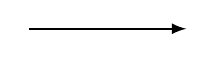
\begin{tikzpicture}[thick] \draw [black,  -latex] (0,6.5) -- (2,6.5); \end{tikzpicture} & 00000000 & 00000001 & \cellcolor[HTML]{FFFFFF}                      & \cellcolor[HTML]{FFFFFF} &                                         \\ \cline{1-1} \cline{3-4}
	\end{tabular}}
	\caption{Permissions table implementation.}
	\label{table:permissions}
\end{table}


\section{Evaluation}
\label{chap:evaluation}

As mentioned in Section \ref{sec:challenges}, the main challenges of this research topic are the portability, speed and security of our proposed system. namely, the OBD-II access control system that is introduced in Chapter \ref{chap:solution}. After introducing the demo implementation in Section \ref{sec:implementation}, it is time to assess whether it meets the aforementioned challenges; proving the feasibility of it's design. This chapter is structured according to our three challenges. First, the overall portability of the system is quantified, by looking at the memory footprint of the software that is deployed on our gateway microcontroller. Second,  we look at the speed it takes to perform the various procedures. Third, the overall security is determined by surveying any potential vulnerabilities. 

\subsection{Portability}
\label{sec:portability}

The portability of our system refers to the ease at which it is introduced in extant vehicle networks. A system that consists of introducing specific hardware, requiring lots of modifications to be made to the vehicle, is unsuitable. Our system consists of introducing additional code to the gateway. In theory, this would consists of simply reprogramming the gateway microcontroller. Granted, the size of the code that enforces the access control system, is bounded by the memory specifications of the gateway. This is why the size of the code that is introduced to the gateway should be kept as small as possible. As an indication, we can take a look at the size of the code of our demo. 

\paragraph{Results}
The total memory footprint (program memory) of our gateway implementation is given in Table \ref{table:portability}. The HMAC\_SHA2 portion refers to the code that implements both SHA hash functions (SHA256 and SHA512), as well as the HMAC\_SHA2 MAC generation and verification algorithms. The ECC portion refers to the code that is used to perform all ECC operations (ECC key pair generation, ECDSA signature verification and ECDH shared secret generation). The last portion (Rest) refers to all other code that is introduced to implement the gateway. Additionally, by analysing the gateway during operation, we saw that no more than 3 Kb is used for data memory at any time (RAM). Non surprisingly, this peak is reached during the computation of the heaviest cryptographic primitive, which is ECC.

\begin{table}[]
	\centering
	\begin{tabular}{|c|c|c|c||c|}
		\hline
		\rowcolor[HTML]{9B9B9B} Type & SHA2 & ECC & Rest (CAN, UART, etc.) & Total \\ \hline
		\cellcolor[HTML]{9B9B9B} Size (KB) & \cellcolor[HTML]{FFFFFF} 2,706 & 18,762 & 10,384 & 31,852 \\ \hline
	\end{tabular}
	\caption{Program memory footprint of implementation on a resource constrained microcontroller.}
	\label{table:portability}
\end{table}

\paragraph{Discussion} The first thing to consider is the data memory (RAM). A peak of 3 Kb is certainly within acceptable bounds, especially if we consider that some automotive gateway microcontrollers that are sold today have a RAM memory of up to several megabytes \cite{GatewayInfineon,GatewayST}. However, it is not unthinkable for some old extant gateway ECU's to lack the necessary RAM to implement our solution. Next, we consider the program memory footprint presented in Table \ref{table:portability}. It should be noted that the total memory footprint of 31,852 Kb is not indicative of the footprint of a real implementation. This is because a typical gateway will have already implemented a lot of functions before introduction of OBD-II RBAC (e.g. CAN object layer). Nonetheless, a total program data size of 31,852 Kb is again within acceptable bounds, since currently sold automotive gateway microcontrollers typically have program memories far exceeding this number \cite{GatewayInfineon,GatewayAtmel,GatewayST}. \\ \\ In short, we can assume that our solution ports well to existing gateway ECU's. There is always a chance that some old gateway microcontroller is not able to support it. Indeed, this chance only increases when older cars are considered, but it is our opinion that this is to be expected.  


\subsection{Speed}
\label{sec:speed}

The speed of our proposed system is of great importance. This is mainly due to the real-time nature of vehicle networks. Messages that are transmitted over different sub-networks, thereby passing through the gateway, need to be delivered as fast as possible. Significant message delays could result in the failure of critical systems (e.g. engine control, ABS, powertrain, etc.). If the authentication scheme proposed in Section \ref{subsec:authenticated_key_agreement_procedure} takes to long to perform, it could cause the gateway to effectively abandon it's other operations. This is also the case for the message authentication procedure presented in Section \ref{subsec:message_authentication_procedure_implementation}. Moreover, a significant delay introduced here could effectively impede the function of the OBD-II interface. This is because a lot of diagnostic and maintenance operations require multiple messages to be sent in sequence. The introduced delays could prohibit the ECU's from recognizing and accepting these sequences. Also, if normal CAN messages are injected to test certain systems, a real-time performance is definitely required here. To evaluate the speed performance of our system, the aforementioned procedures are key. 

\paragraph{Results}
We've mentioned before that asymmetric cryptographic operations are computationally hard to perform; especially on platforms with limited processing power, as is the case here. The authenticated key agreement procedure of our proposed system introduces three ECC operations performed on the gateway: Generating a new public key pair (KGen), Verifying the signature that is received from the tester (Ver), and the generation of the shared secret (ECDH). The message authentication procedure only includes one significant cryptographic operation: the MAC verification (Ver). The performance of all of these procedures is given in Table \ref{table:eval1}. We skipped over the operations that are performed by the tester (calling the central server for the signature, as well as also generating a shared secret). This is because any tester device would be designed with these operations in mind, introducing dedicated hardware that allows fast and efficient shared secret generation. As well as a fast and secure way of interfacing with the central server. We also omitted the time it takes to send the CAN messages themselves. Considering our CAN controller is set to a baud rate of 125 Kbps, we can use \cite{CANspeed} to calculate that every message takes roughly 1.04 milliseconds to transmit. This indicates that the performance of our design is dominated by the cryptographic operations that were introduced, rather than the amount of transmitted CAN messages.  
\begin{table}[]
	\adjustbox{max width=\textwidth}{%
	\begin{tabular}{|c|ccc||c|}
		\hline
		\rowcolor[HTML]{9B9B9B} Procedure & Authenticated & Key & Agreement & Message Authentication \\ \hline
		\cellcolor[HTML]{9B9B9B} Cryptographic Operation & \multicolumn{1}{c|}{\cellcolor[HTML]{FFFFFF} KGen } & \multicolumn{1}{c|}{Ver (ECDSA)} & ECDH & Ver (MAC) \\ \hline
		\cellcolor[HTML]{9B9B9B} Performance (seconds) & \multicolumn{1}{c|}{8,593} & \multicolumn{1}{c|}{10,16} & 8,565 & 0,124 \\ \hline
	\end{tabular}}
	\caption{Performance of cryptographic operations on a resource constrained microcontroller.}
	\label{table:eval1}
\end{table}

\paragraph{Discussion} The first takeaway from the results of our evaluation presented in Table \ref{table:eval1}, is that the cryptographic operations of the authenticated key agreement procedure take long to perform; each one taking roughly 9 seconds to complete. This in line with our expectations, since we know that asymmetric key operations are computationally very intensive. Indeed, if we compare them to the symmetric key operation performed in the message authentication procedure, which takes only 124 milliseconds, this distinction becomes even more apparent. Remember that the decision was made to use a resource constrained microcontroller, with a CPU clock speed of only 8 MHz and word size of 8 bits. Actual automotive gateway microcontrollers that are sold today have clock speeds ranging from 8 up to 300 MHz and word sizes of 8, 16, or 32 bits \cite{GatewayInfineon,GatewayAtmel,GatewayST}. Some of these even incorporate hardware accelerators for ECC and SHA2 operations \cite{GatewayInfineon}. Therefore, if our solution were implemented on real automotive gateways, our performance would likely increase. Nonetheless, the time it takes to complete the authenticated key agreement procedure is significant. If a gateway were to initiate this sequence while in operation (i.e. the car is driving), all internal network communications would have to be postponed for roughly 30 seconds, which would be disastrous. To solve this issue, we assert that internal network communications should have precedence over the OBD-II authentication procedure. This means that the system could reject any OBD-II authentication attempts while driving. Alternatively, an interrupt can be generated every time an internal message is received, postponing the authentication procedure until the message is handled. This scenario becomes increasingly likely when we consider that a lot of modern ECU's provide a dual-processor with service separation \cite{GatewayPerformance}. Here, a dedicated processor would handle incoming messages, thereby preventing the OBD-II procedures from interfering. \\ \\ While the running times of the authentication procedure are long, they are only required for the initial authentication. Once this is done, the message authentication procedure takes over. This procedure introduces three delays: the signature generation on the tester, the permissions check and the MAC verification (we mentioned earlier that message transmission times are not considered). Signature generation doesn't incur any real delay, since the tester would generate the signature, and send the message and the signature back-to-back. Since every CAN ID is finite (i.e. 11 bits for our demo), every permission table lookup can be completed in constant time, so this delay is take out of consideration as well. We can conclude that the performance of the message authentication procedure is dominated by the MAC verification, which takes only 124 milliseconds. \\ \\ To conclude, the design of our solution is feasible in terms of performance. However, the authenticated key agreement procedure is slow, and if performed in one pass, would indeed impede the operation of the internal network. This is why care must be taken not to let the OBD-II authentication procedure interfere with internal communications/ This can be facilitated in two ways: rejecting OBD-II authentication while driving or decoupling OBD-II RBAC operations from other gateway functions by using interrupts or dual-processing technologies. 


\subsection{Security}
\label{sec:security}

The most intrinsic property of any RBAC system is it's security, and OBD-II access control is certainly no exception. The goal of our system is to curtail the wide open nature of the OBD-II interface; forcing individuals to garner the right credentials, before access is granted. If the procedures that were introduced to enforce these goals are flawed, thereby allowing them to be easily bypassed, the design of our system has critically failed. To systematically evaluate the security of our system, we will attempt to survey any potential weaknesses.


\paragraph{Cryptographic Primitives} An obvious potential weakness of our system is the cryptographic primitives themselves: the ECC keys and operations, the hash functions and of course the MAC verification process. A weakness in any of these would present a significant security breach. Imagine if the ECC signatures could be easily calculated without possession of the appropriate private key. Or if MAC messages could be replayed in an effort to hijack extant sessions. To guarantee the security of these primitives, three things need to be assured. First, the original design should universally be considered sound and secure, allowing them to be used in professional applications. Luckily this is the case for all the primitives included in our solution: all ECC operations, HMAC\textunderscore SHA256 and SHA512. Second, the size of the keys and signatures should be sufficiently large. Again, this is the case since all of them were chosen to guarantee a security level of 128 bits. Third, the implementation of these primitives should not contain any flaws, allowing them to be broken. The burden of guaranteeing this lies with the OEM's themselves, since they would eventually be implementing them in vehicles all over the world. 

\paragraph{Authenticated Key Agreement Procedure}
Remember from Section \ref{sec:attacker_model} that we consider two basic attack scenarios: an attacker directly interfacing with the OBD-II port (Figure \ref{fig:attackmodel_1}) and an attacker hijacking an extant session remotely (Figure \ref{fig:attackmodel_2}). The first scenario is directly linked with the authentication procedure. This procedure was based on the ECDHE\textunderscore ECDSA procedure introduced in \cite{RFC4492}, so it's safe to assume our design inherits the same security guarantees. However, we did introduce some changes; we need to make sure these changes do not jeopardise the overall security of the procedure. Next, we take a look at these changes one-by-one, ensuring they are harmless.
\begin{itemize}
	\item \textbf{Gateway Key Pair:} The generation of a new ECC key pair was introduced on the gateway since both parties require a key pair for the ECDH operations. The only difference with the original ECDHE\textunderscore ECDSA system is that this pair is generated on the fly for the gateway. When generating this key pair, it must be assured that they are random. If they were not, this would allow individuals to predict them. The problem of random number generation is discussed in the next paragraph.
	
	\item \textbf{Perfect Forward Secrecy:} We already discussed why PFS is not a concern for our system. Omitting the ephemeral key pairs results in a more efficient system without having an adverse effect on it's security.
	
	\item \textbf{Mutual Authentication:} The omission of two way authentication is necessary because of the initial absence of an ECC key pair on the gateway. In the end, the only security property that is lost here is authentication of the gateway, which is not necessary since the user should be aware whether (s)he is interfacing with a legitimate gateway or not.
\end{itemize} 

\paragraph{Random Number Generation} As mentioned before, a sound random number generator (RNG) is essential to the security of our system. RNG's are difficult to implement because of the deterministic nature of computers. A software RNG with a known seed will always generate the same sequence of numbers, allowing them to be predicted when the RNG procedure and seed are known (e.g. by reverse engineering the gateway). This is why it is often implemented by using sources that are inherently unpredictable: the noise on a network bus, the value of a sensor, the contents of an arbitrary memory location, etc. Hash functions can also be useful here to provide an extra layer of entropy. 

\paragraph{Message Authentication Procedure}
The message authentication procedure is more concerned with our second attack scenario; namely, remote session hacking. This is because the MAC's were introduced to ensure that the messages were transmitted by the authenticated user (i.e. the user that successfully performed the authentication procedure). Our procedure follows the general structure of any MAC system: a message is sent together with a MAC of the message. Any adversary that has the ability to read and inject messages into this session is limited in terms of attack capabilities. Altering extant messages is impossible, since this would invalidate the MAC. Injecting messages is also impossible since the attacker would have to generate a MAC, and this requires knowledge of the session key. They could flood the system with messages to shut down the session. Or intercept valid messages that were sent by the user. These problems can only be solved by securing the remote connection itself.  

\paragraph{Central Server Connection} With the introduction of the central server, we have unintentionally introduced a third attack vector: the connection to the central server. If these connection were insecure, it would allow third parties to monitor and interfere with the signature transmission. While this may seem harmless, it does open up the ability of systematically collecting signature/public key pairs for a specific car model, allowing them to be replayed in the future whenever the same public key is generated. Luckily, the cost in terms of time and effort is immense, which might prevent anyone from ever attempting it. Nonetheless, a secure internet connection is certainly a must.

\paragraph{Private Key Disclosure} It is essential that the OBD-II private keys are securely stored on the central server. Disclosure of these keys would invalidate the entire system, requiring the introduction of new public keys in all vehicles that support our solution. Luckily, secure servers are commonplace on the internet, so it's just a matter of employing the appropriate technologies. Besides the OBD-II private keys, there's also the private key that is generated on the gateway, as well as the shared secret. We do not protect against physical access, so an adversary analysing a gateway and extracting the newly generated private key is possible (although it seems futile, since physical access would allow the attacker to bypass the RBAC system altogether). Only protected memory architectures would solve this issue. However, if a software vulnerability is introduced that discloses the private key or session key on the CAN bus, this would be disastrous and should be avoided at all times.

\paragraph{Permission Table} The permission table introduces the same issue as before. If someone has physical access to the gateway, (s)he can modify the permissions table. Again this attack is only solvable by introducing sections of protected memory. The system will undoubtedly include admin messages that are designed to modify the security policy (i.e. the permissions table). If an attacker is able to successfully transmit these messages, it would mean the OBD-II port is wide open once more.

\chapter{Conclusion}
The last chapter of this thesis paper consists of two main parts. First, the contribution presented in section \ref{sec:contributions} is reviewed and discussed. Second, we present a couple of areas where additional research is required, as well as why this is the case.

\section{Contribution in Review}
The contribution presented in section \ref{sec:contributions} consists of two assertions. First, the proposal of a role-based access control model for OBD-II that is based on public key cryptography. Second, providing an implementation of this model on a resource-constrained ECU that is evaluated in terms of portability, speed and security. \\ \\ The first assertion corresponds with the solution that is proposed in section \ref{chap:solution}. While limited in scope (i.e. no protection against physical access), this solution does exactly what it was designed for: protecting the OBD-II interface. By introducing this solution to the gateway, there is no way for any OBD-II connection to circumvent it. By storing the public keys on the gateway and the private keys on a central server, key disclosure problems are limited. And, by introducing the central server, it is feasible for anyone to initiate an OBD-II session. As long as they are in possession of the right credentials, as well as a working internet connection. The procedures that were introduced to facilitate these authenticated sessions are state of the art (e.g. ECC), and are based on other well-known and often used designs (e.g. ECDHE\textunderscore ECDSA, which is used in TLS). \\ \\ The second assertion corresponds with the implementation and evaluation presented in section \ref{chap:implementation}. While the microcontrollers that we used in our implementation are not automotive ECU's, they closely match their specifications in terms of architecture and performance (e.g. 8 bit AVR). The technical difficulties of implementing a lightweight security procedure based on public key cryptography, are the same for both types of hardware (e.g. limited processing power, limited memory, etc.). This is why our implementation should be considered a proof of concept of OBD-II security for the automotive industry. Moreover, in section \ref{chap:evaluation} this implementation is successfully evaluated in terms of portability, speed and security. It is therefore safe to assume that our solution ports well to extant vehicle networks, while guaranteeing the same level of security that our implementation did. Which is exactly what we set out to do with this thesis paper.

\section{Future Research}
The contribution of this thesis paper is from all-encompassing. The extensive nature of our problem statement attributes to a series of areas that require additional research. This thesis is concluded with a presentation of different topics that merit a research paper of their own.

\begin{itemize}
	\item \textbf{OBD-II Roles:} In section \ref{subsec:sol_permissions_table} a series of possible roles are presented. However, these were only based on the literature study performed by the researchers of this paper. Additional research, incorporating input from various stakeholders (e.g. car manufacturers, the government, repairmen, etc.) would undoubtedly result in a more fine-grained specification. One that more closely adheres to the current automotive industry landscape.
	
	\item \textbf{Permissions Table:} The permission table implementation presented in section \ref{subsec:permissions_table_implementation} was designed only for testing purposes. A real implementation would have to incorporate a real permissions table; one that is designed to protect extant intra vehicle networks. This requires input from automotive network professionals (e.g. car manufacturers and OEM's).
	
	\item \textbf{Central Server} Up to know, only the goal of this server is well-defined: securely store the appropriate private keys, supplying a API for private key procedures and allowing for users to authenticate to the server. A lot of additional questions remain to be answered: What hardware should be used? Who should manage these servers? who should pay for them? where should they be built? How to implement the private key API? etc. It is essential that these questions are answered by performing additional research.
	
	\item \textbf{Tester and OBD-II applications} For our system to be feasible, it is essential that everyone has access to the appropriate tools. This tool is of course the tester device or a OBD-II application for personal computers. While the function of these is well-defined (performing the authentication procedures and interfacing with the central server), how these are designed, manufactured and distributed remains to be seen. If our solution is widely implemented, there's a significant monetary incentive for third parties to start developing tester devices as well as OBD-II applications for personal computers. Nonetheless, additional research is definitely required.
\end{itemize}


\backmatter

\bibliographystyle{plainurl}
\bibliography{references}

\end{document}

